%%%%%%%%%%%%%%%%%%%%%%%%%%%%%%%%%%%%%%%%%%%%%%%
%
% Template per Elaborato di Laurea
% DISI - Dipartimento di Ingegneria e Scienza dell’Informazione
%
% update 2015-09-10
%
% Per la generazione corretta del 
% pdflatex nome_file.tex
% bibtex nome_file.aux
% pdflatex nome_file.tex
% pdflatex nome_file.tex
%
%%%%%%%%%%%%%%%%%%%%%%%%%%%%%%%%%%%%%%%%%%%%%%%

% formato FRONTE RETRO
\documentclass[a4paper,11pt,titlepage,twoside,openany]{book}
\usepackage{plain}
\usepackage{setspace}
\usepackage[paperheight=29.7cm,paperwidth=21cm,outer=1.5cm,inner=2.5cm,top=2cm,bottom=2cm]{geometry} % per definizione layout
\usepackage{titlesec} % per formato custom dei titoli dei capitoli
\usepackage{url}
\usepackage{graphicx}
\usepackage{wrapfig}
\usepackage[italian]{varioref}
\usepackage{booktabs}
\usepackage{bera}% optional: just to have a nice mono-spaced font
\usepackage{listings}
\usepackage{xcolor}
\usepackage{multicol}
%%%%%%%%%%%%%%
% supporto lettere accentate
%
%\usepackage[latin1]{inputenc} % per Windows;
\usepackage[utf8x]{inputenc} % per Linux (richiede il pacchetto unicode);
%\usepackage[applemac]{inputenc} % per Mac.

\colorlet{punct}{red!60!black}
\definecolor{background}{HTML}{EEEEEE}
\definecolor{delim}{RGB}{20,105,176}
\colorlet{numb}{magenta!60!black}
\lstdefinelanguage{json}{
    basicstyle=\normalfont\ttfamily,
    numbers=left,
    numberstyle=\scriptsize,
    stepnumber=1,
    numbersep=8pt,
    showstringspaces=false,
    breaklines=true,
    frame=lines,
    literate=
     *{0}{{{\color{numb}0}}}{1}
      {1}{{{\color{numb}1}}}{1}
      {2}{{{\color{numb}2}}}{1}
      {3}{{{\color{numb}3}}}{1}
      {4}{{{\color{numb}4}}}{1}
      {5}{{{\color{numb}5}}}{1}
      {6}{{{\color{numb}6}}}{1}
      {7}{{{\color{numb}7}}}{1}
      {8}{{{\color{numb}8}}}{1}
      {9}{{{\color{numb}9}}}{1}
      {:}{{{\color{punct}{:}}}}{1}
      {,}{{{\color{punct}{,}}}}{1}
      {\{}{{{\color{delim}{\{}}}}{1}
      {\}}{{{\color{delim}{\}}}}}{1}
      {[}{{{\color{delim}{[}}}}{1}
      {]}{{{\color{delim}{]}}}}{1},
}

\singlespacing

\usepackage[italian]{babel}

\begin{document}

  % nessuna numerazione
  \pagenumbering{gobble} 
  \pagestyle{plain}

\thispagestyle{empty}

\begin{center}
  \begin{figure}[h!]
    \centerline{
      
\includegraphics[width=0.6\textwidth]{chapters/titlepage/assets/marchio_unitrento_colore_it_v2.eps}
    }
  \end{figure}

  \vspace{2 cm} 

  \LARGE{Dipartimento di Ingegneria e Scienza dell’Informazione\\}

  \vspace{1 cm} 
  \Large{Corso di Laurea in\\
    Informatica
    %Ingegneria dell'Informazione e delle Comunicazioni
    %Ingegneria dell'Informazione e Organizzazione d'Impresa
    %Ingegneria Elettronica e delle Telecomunicazioni
  }

  \vspace{2 cm} 
  \Large\textsc{Elaborato finale\\} 
  \vspace{1 cm} 
  \Huge\textsc{Titolo\\}
  \Large{\it{Sottotitolo (alcune volte lungo - opzionale)}}


  \vspace{2 cm} 
  \begin{tabular*}{\textwidth}{ c @{\extracolsep{\fill}} c }
  \Large{Supervisore} & \Large{Laureando}\\
  \Large{Prof. Alberto Montresor}& \Large{Filippo Momesso}\\
  \end{tabular*}

  \vspace{2 cm} 

  \Large{Anno accademico 2020/2021}
  
\end{center}



  \clearpage
 
%%%%%%%%%%%%%%%%%%%%%%%%%%%%%%%%%%%%%%%%%%%%%%%%%%%%%%%%%%%%%%%%%%%%%%%%%%
%%%%%%%%%%%%%%%%%%%%%%%%%%%%%%%%%%%%%%%%%%%%%%%%%%%%%%%%%%%%%%%%%%%%%%%%%%
%% Nota
%%%%%%%%%%%%%%%%%%%%%%%%%%%%%%%%%%%%%%%%%%%%%%%%%%%%%%%%%%%%%%%%%%%%%%%%%%
%% Sezione Ringraziamenti opzionale
%%%%%%%%%%%%%%%%%%%%%%%%%%%%%%%%%%%%%%%%%%%%%%%%%%%%%%%%%%%%%%%%%%%%%%%%%%
%%%%%%%%%%%%%%%%%%%%%%%%%%%%%%%%%%%%%%%%%%%%%%%%%%%%%%%%%%%%%%%%%%%%%%%%%%
  \thispagestyle{empty}

\begin{center}
  {\bf \Huge Ringraziamenti}
\end{center}

\vspace{4cm}

\textit{
  Innanzitutto voglio esprimere la mia sincera gratitudine nei confronti del Professor Alberto Montresor, il quale si è prestato a svolgere il ruolo di relatore di questa tesi e mi ha seguito durante il tirocinio.}

\textit{
  Grazie alla mia famiglia, che mi ha sempre sostenuto e incoraggiato in ogni mia singola attività e in particolare nello studio. Grazie Mamma, Papà e Riccardo.}


\textit{  
  Agli amici e ai compagni di corso, che tra un meme e l'altro, sono sempre stati presenti quando era necessario risolvere qualche bug o passare qualche esame ostico.}

\textit{  
  Grazie infine a te, Giada, che mi fai stare bene da quando, ormai quasi cinque anni fa, sei entrata nella mia vita.
}
\vspace{2 cm} 
\begin{flushright}
  Filippo Momesso
\end{flushright} 

\newpage
\thispagestyle{plain} % empty
\mbox{}
  \clearpage
  \pagestyle{plain} % nessuna intestazione e pie pagina con numero al centro

  
  % inizio numerazione pagine in numeri arabi
  \mainmatter

%%%%%%%%%%%%%%%%%%%%%%%%%%%%%%%%%%%%%%%%%%%%%%%%%%%%%%%%%%%%%%%%%%%%%%%%%%
%%%%%%%%%%%%%%%%%%%%%%%%%%%%%%%%%%%%%%%%%%%%%%%%%%%%%%%%%%%%%%%%%%%%%%%%%%
%% Nota
%%%%%%%%%%%%%%%%%%%%%%%%%%%%%%%%%%%%%%%%%%%%%%%%%%%%%%%%%%%%%%%%%%%%%%%%%%
%% Si ricorda che il numero massimo di facciate e' 30.
%% Nel conteggio delle facciate sono incluse 
%%   indice
%%   sommario
%%   capitoli
%% Dal conteggio delle facciate sono escluse
%%   frontespizio
%%   ringraziamenti
%%   allegati    
%%%%%%%%%%%%%%%%%%%%%%%%%%%%%%%%%%%%%%%%%%%%%%%%%%%%%%%%%%%%%%%%%%%%%%%%%%
%%%%%%%%%%%%%%%%%%%%%%%%%%%%%%%%%%%%%%%%%%%%%%%%%%%%%%%%%%%%%%%%%%%%%%%%%%

    % indice
    \tableofcontents
    \clearpage
    
    
          
    % gruppo per definizone di successione capitoli senza interruzione di pagina
    \begingroup
      % nessuna interruzione di pagina tra capitoli
      % ridefinizione dei comandi di clear page
      \renewcommand{\cleardoublepage}{} 
      \renewcommand{\clearpage}{} 
      % redefinizione del formato del titolo del capitolo
      % da formato
      %   Capitolo X
      %   Titolo capitolo
      % a formato
      %   X   Titolo capitolo
      
      \titleformat{\chapter}
        {\normalfont\Huge\bfseries}{\thechapter}{1em}{}
        
      \titlespacing*{\chapter}{0pt}{0.59in}{0.02in}
      \titlespacing*{\section}{0pt}{0.20in}{0.02in}
      \titlespacing*{\subsection}{0pt}{0.10in}{0.02in}
      
      % sommario
      %\chapter*{Sommario} % senza numerazione
\label{sommario}

\addcontentsline{toc}{chapter}{Sommario} % da aggiungere comunque all'indiceù
Questo elaborato descrive il lavoro svolto dal laureando Momesso Filippo durante l'attività di tirocinio formativo. Lo stage ha avuto una durata di 225 ore e si è svolto presso l'azienda Cluster Reply Srl, nella sede di Silea (TV). Tuttavia, viste le restrizioni imposte dalle istituzioni a causa della pandemia da Covid-19, l'attività lavorativa si è svolta da remoto.

Durante il tirocinio, il laureando ha sviluppato due progetti finalizzati all'automazione di flussi di business utilizzando Microsoft Dynamics 365, Microsoft Power Automate e Microsoft AI Builder. Per lo sviluppo delle due soluzioni software, è stata necessaria una customizzazione a \num{360} gradi, utilizzando sia le funzionalità low-code/no-code che lo sviluppo di plug-in in linguaggio C\# e l'SDK Microsoft XRM. 

Il primo capitolo tratta il contesto aziendale, con un approfondimento sulle metodologie lavorative, la struttura dei team di lavoro e gli strumenti di Cluster Reply. Nel secondo capitolo, viene effettuata un'analisi nel dettaglio delle tecnologie Microsoft apprese e utilizzate dal tirocinante durante il periodo di stage. 
Il terzo e il quarto capitolo descrivono i progetti sviluppati mentre nel quinto viene effettuata un'analisi complessiva sull'esperienza di tirocinio. 

Lo stage formativo ha permesso al laureando di completare il percorso di laurea con un esempio reale del funzionamento del mondo del lavoro nel settore IT, oltre che apprendere nuove tecnologie che, di norma, difficilmente vengono affrontate durante il Corso di Laurea in Informatica. Pertanto l'esperienza è risultata più che positiva. 
\newpage


%%%%%%%%%%%%%%%%%%%%%%%%%%%%%%%%%%%%%%%%%%%%%%%%%%%%%%%%%%%%%%%%%%%%%%%%%%
%%%%%%%%%%%%%%%%%%%%%%%%%%%%%%%%%%%%%%%%%%%%%%%%%%%%%%%%%%%%%%%%%%%%%%%%%%
%% Nota
%%%%%%%%%%%%%%%%%%%%%%%%%%%%%%%%%%%%%%%%%%%%%%%%%%%%%%%%%%%%%%%%%%%%%%%%%%
%% Sommario e' un breve riassunto del lavoro svolto dove si descrive 
%% l’obiettivo, l’oggetto della tesi, le metodologie e 
%% le tecniche usate, i dati elaborati e la spiegazione delle conclusioni 
%% alle quali siete arrivati.
%% Il sommario dell’elaborato consiste al massimo di 3 pagine e deve contenere le seguenti informazioni: 
%%   contesto e motivazioni
%%   breve riassunto del problema affrontato
%%   tecniche utilizzate e/o sviluppate
%%   risultati raggiunti, sottolineando il contributo personale del laureando/a
%%%%%%%%%%%%%%%%%%%%%%%%%%%%%%%%%%%%%%%%%%%%%%%%%%%%%%%%%%%%%%%%%%%%%%%%%%
%%%%%%%%%%%%%%%%%%%%%%%%%%%%%%%%%%%%%%%%%%%%%%%%%%%%%%%%%%%%%%%%%%%%%%%%%%      
      
      %%%%%%%%%%%%%%%%%%%%%%%%%%%%%%%%
      % lista dei capitoli
      %
      % \input oppure \include
      %
      \graphicspath{{./chapters/01/assets/} }
\chapter{Contesto Aziendale}
\label{cha:intro}

\section{Il gruppo Reply}
Reply è una società specializzata in consulenze, \textit{system integration} e servizi digitali con un focus sulla concezione, design e implementazione di soluzioni basate sulle nuove tecnologie e i nuovi canali di comunicazione. Operativa dal 1996, collabora dunque con importanti realtà aziendali di diversi settori al fine di definire e sviluppare modelli di business resi possibili dai nuovi paradigmi tecnologici quali \textit{Artificial Intelligence}, \textit{Big Data}, \textit{Cloud Computing}, \textit{Digital Communication}, \textit{Internet of Things} e \textit{Social Networking}.
Il campo di azione di Reply è quello delle aziende dei settori bancario e finanziario, industriale e dei servizi, delle telecomunicazioni, dell'energia e della pubblica amministrazione.
I principali servizi offerti da Reply sono:
\begin{itemize}
  \item \textbf{Consulenze} su strategie, comunicazione, processi aziendali e tecnologie;
  \item \textbf{\textit{System Integration}} di soluzioni software esistenti;
  \item \textbf{Gestione}, monitoraggio e sviluppo continuo di sistemi e applicazioni software.
\end{itemize}

Il gruppo è formato da decine di società secondo un modello a rete e nel corso degli anni si è conquistato una posizione di prestigio nel panorama europeo e mondiale. Il fatturato 2020 si attesta a 1.250,2 milioni di Euro \cite{fatturato}.

\section{Cluster Reply}

\begin{figure}[h]
  \centering
  
\includegraphics[width=0.35\textwidth]{logo-cluster-reply.png}
  \caption{Logo Cluster Reply Srl}
  \label{fig:replyClusterLogo}
\end{figure}

Cluster Reply è la società del gruppo Reply specializzata in servizi di consulenza e di integrazione di sistemi su tecnologie Microsoft. Opera in Italia in collaborazione con le altre aziende del gruppo specializzate in tecnologie Microsoft. È presente sul territorio con sedi a Milano, Padova, Roma, Torino, Trieste, Bologna e Silea. 

Per quanto riguarda la struttura, Cluster Reply è divisa in diverse sezioni, ognuna dedicata a uno specifico settore di business. Si ha una sezione dedicata a Microsoft Azure, una al sistema Microsoft ERP (\textit{Enterprise Resource Planning}), una al settore \textit{Manifacturing}, una al settore \textit{Financial} (banche e assicurazioni) e infine una sezione dedicata alla \textit{Customer Experience}.

È in quest'ultima sezione che ho svolto la mia attività di tirocinio formativo. Essa è altamente specializzata nella consulenza e realizzazione di sistemi custom basati su Microsoft Dynamics 365, la linea di applicazioni aziendali intelligenti per la pianificazione di risorse aziendali e la gestione delle relazioni con i clienti. Di questa ampia gamma di prodotti, durante il tirocinio ho avuto la possibilità di approfondire la conoscenza delle applicazioni CRM (\textit{Customer Relationship Management}) Sales Hub, Cucstomer Service Hub e un'applicazione custom specifitacamente sviluppata per un cliente.

\section{Progetti, Clienti e Prodotti}
Tra i progetti più importanti dell'azienda (non coperti da segreto professionale) si può menzionare il "sistema di automazione delle attività nella gestione degli affitti arretrati" sviluppato per il cliente Notting Hill Genesis. La soluzione proposta da Cluster Reply consiste di una soluzione CRM basata sulla piattaforma Microsoft Dynamics 365 per l'automazione  delle attività degli utenti e la comunicazione verso i clienti. Questa soluzione permette la gestione di un flusso automatizzato per la gestione degli affitti arrettrati, in grado di guidare gli utenti NHG e automatizzare le comunicazioni (SMS, email e lettere) verso i clienti, gestendone le tempistiche, i template dinamici da utilizzare e salvando l'intera documentazione su Microsoft SharePoint in caso di rinvio legale \cite{NHG}.

Un'altro prodotto confezionato e pubblicato sul Microsoft Store da Cluster Reply è il motore di configurazione di Workflow “Configurable Workflow \& SLAs Engine”. Grazie a questo prodotto software da integrare in Microsoft Dynamics 365 è possibile semplificare la configurazione e la gestione dei \textit{workflow} e degli SLA (\textit{Service Level Agreement}) \cite{configurableWorkflow}.




      \graphicspath{{./chapters/02/assets/}}

\chapter{Analisi delle tecnologie}
In questo capitolo viene effettuata un'analisi dettagliata delle tecnologie Microsoft apprese e utilizzate durante il tirocinio.

\section{Microsoft Dynamics CRM}

Microsoft Dynamics CRM\footnote{Devo davvero ringraziare Tutorialspoint perché la sua guida~\cite{DynamicsTutorialspoint}, su cui mi sono basato per l'elaborazione di questa sezione, mi ha chiarito moltissimi dubbi che la documentazione ufficiale (estremamente confusionaria) e i colleghi in azienda non sono riusciti a risolvermi.} è un pacchetto software per la gestione delle relazioni con il cliente sviluppato da Microsoft. Seppure interamente customizzabile grazie al framework proprietario Microsoft XRM SDK basato su .NET, di base si concentra sui settori Vendite, Marketing e Servizio Clienti.

Il CRM può essere infatti utilizzato per aumentare la produttività delle vendite e l'efficacia del marketing per un'azienda, gestire l'intera catena di assistenza clienti e fornire informazioni sull'andamento dei social media, business intelligence e molte altre caratteristiche e funzionalità pronte all'uso.
L'interazione utente con Microsoft Dynamics CRM avviene attraverso l'interfaccia web, la quale è ottimizzata anche per l'utilizzo mobile e tablet oltre che desktop.

\subsection{Moduli Funzionali}
Il CRM è interamente progettato sui moduli funzionali Sales, Marketing e Service Management. Questa divisione in moduli è dovuta al fatto che un'azienda, nell'utilizzare il CRM per gestire i propri processi, necessita che gli utenti del settore vendite, ad esempio, abbiano a disposizione delle funzionalità specifiche disponibili nel modulo Sales, parimenti gli utenti del settore marketing con il modulo Marketing e gli utenti del servizio clienti con il modulo Service Management.

\subsubsection{Modulo Sales}
Il modulo Sales del CRM è progettato per gestire l'intero ciclo di vita di un nuovo cliente. Si compone dei seguenti sotto-moduli:
\begin{itemize}
  \item \textbf{Leads} - Rappresenta una persona o un'organizzazione che può diventare un potenziale cliente. Questo è il primo passaggio per l'inserimento di un potenziale cliente nel sistema.
  \item \textbf{Opportunities} - Rappresenta una potenziale vendita al cliente. Quando un Lead mostra interesse nell'offerta, viene convertita in Opportunity. Un'Opportunity può essere vinta o persa.
  \item \textbf{Accounts} - Rappresenta un'azienda con cui si ha una relazione. Quando un'Opportunity è vinta, viene convertita in un Account o un Contact.
  \item \textbf{Contacts} - Rappresenta una persona o un individuo con cui l'azienda ha una relazione. In genere, un Contact è un cliente (ad esempio tutti gli intestatari di un conto presso per una banca).
  \item \textbf{Competitors} - Gestisce i concorrenti di mercato dell'azienda.
  \item \textbf{Products} - Gestisce i prodotti offerti dall'azienda ai clienti.
  \item \textbf{Quotes} - Preventivo formale di prodotti o servizi proposti a prezzi specifici a un potenziale cliente.
  \item \textbf{Orders} - Quando un Quote viene accettato da un cliente viene convertito in un Order.
  \item \textbf{Invoices} - Fattura generata da un ordine.
\end{itemize}

\subsubsection{Modulo Marketing}
Il modulo Marketing del CRM è progettato per gestire l'intero processo di marketing di un'azienda per i suoi clienti esistenti e potenziali. Si compone dei seguenti sotto-moduli, i quali funzionano in coordinazione con il modulo Sales:
\begin{itemize}
  \item \textbf{Marketing Lists} - Fornisce un metodo per raggruppare Contact, Account e Lead e interagire con essi attraverso l'invio di email promozionali, dettagli di eventi, newsletter e altre comunicazioni rilevanti per il cliente. È possibile definire dei criteri per creare le Marketing List.
  \item \textbf{Campaigns} - Servono a misurare l'efficacia e il completamento di uno specifico risultato, come l'introduzione di un nuovo prodotto o l'incremento della quota di mercato e può includere diversi canali di comunicazione come email e altre forme pubblicitarie.
  \item \textbf{Quick Campaigns} - Simile a una Campaign ma può essere messa in relazione con un solo tipo di Activity\footnote{Vedi sottosezione Gestione attività.}.
\end{itemize}

\subsubsection{Modulo Service}
Il modulo Service del CRM è progettato per gestire e tracciare le operazioni di servizio clienti di un'azienda come il supporto ai servizi basati su incidenti/casi, pianificazione di interventi di supporto ai clienti, eccetera. Si compone dei seguenti sotto-moduli:
\begin{itemize}
  \item \textbf{Cases} - Permette di tracciare una qualsiasi richiesta, problema o lamentela di un cliente. Un Case ha un processo di risoluzione composto di vari stati che terminano con la risoluzione o la chiusura del Case.
  \item \textbf{Knowledge Base} - Mantiene una collezione d tutte le domande e risposte più comuni.
  \item \textbf{Contracts} - In relazione con Cases indica i contratti attivi del cliente.
  \item \textbf{Resources/Resouce Groups} - Rappresenta le persone, strumenti, luoghi o l'attrezzatura necessaria per fornire un servizio. Possono essere utilizzate per risolvere uno specifico problema di un cliente.
  \item \textbf{Services} - Rappresentano i servizi di assistenza che l'azienda offre ai clienti.
  \item \textbf{Service Calendar} - Permette di organizzare le operazioni di assistenza.
\end{itemize}

\subsubsection{Gestione attività}
\label{sssec:gestione-attivita}
Tutti i moduli precedentemente trattati fanno uso del modulo Activity Management del CRM. Un'\textit{activity} rappresenta qualsiasi tipo di interazione con il cliente come telefonate, email, lettere, appuntamenti e altro ancora. Queste \textit{activity} possono essere messe in relazione con le altre entità trattate precedentemente appartenenti ai vari moduli del CRM.

\subsection{Entità e Record}
Un'\textit{entità} è utilizzata per modellare dei dati nel CRM. Contact, Case, Account e Lead sono tutte entità del CRM che possono essere istanziate in record. A livello concettuale un'entità è equivalente a una tabella di un database relazionale.

Oltre alle entità presenti di default nel CRM è possibile definire nuove entità custom in base alle necessità specifiche, oppure modificare quelle esistenti aggiungendo o eliminando campi.

Il CRM fornisce undici tipi di campi:
\begin{itemize}
  \item Single Line of Text
  \item Option Set (Dropdown)
  \item Two Options (Radio Button)
  \item Image
  \item Whole Number
  \item Floating Point Number
  \item Decimal Number
  \item Currency
  \item Multiple Lines of Text
  \item Date and Time
  \item Lookup
\end{itemize} 

A partire dalla versione 2011 inoltre è disponibile un particolare tipo di campo chiamato Party List. Questo tipo consente di mappare una relazione tra entità come nel caso del tipo Lookup ma con la differenza che quest'ultimo può mappare una relazione con una singola entità mentre un campo di tipo Party List permette di avere una relazione con entità multiple. Per esempio, una email può essere associata a un Contact, un User o una Queue.

\subsection{Moduli (Forms)}
Per creare, aggiornare o modificare un record nel CRM si utilizzano i Form. Ad ogni entità possono dunque essere associati uno o più Form. A seconda dell'opzione di visualizzazione scelta, del modulo funzionale selezionato o del tipo di utente che interagisce con il CRM possono essere visualizzati Form diversi. 
I form possono essere creati attraverso un'interfaccia apposita presente nelle impostazioni di customizzazione del CRM.
\begin{figure}[ht!]
  \centering
  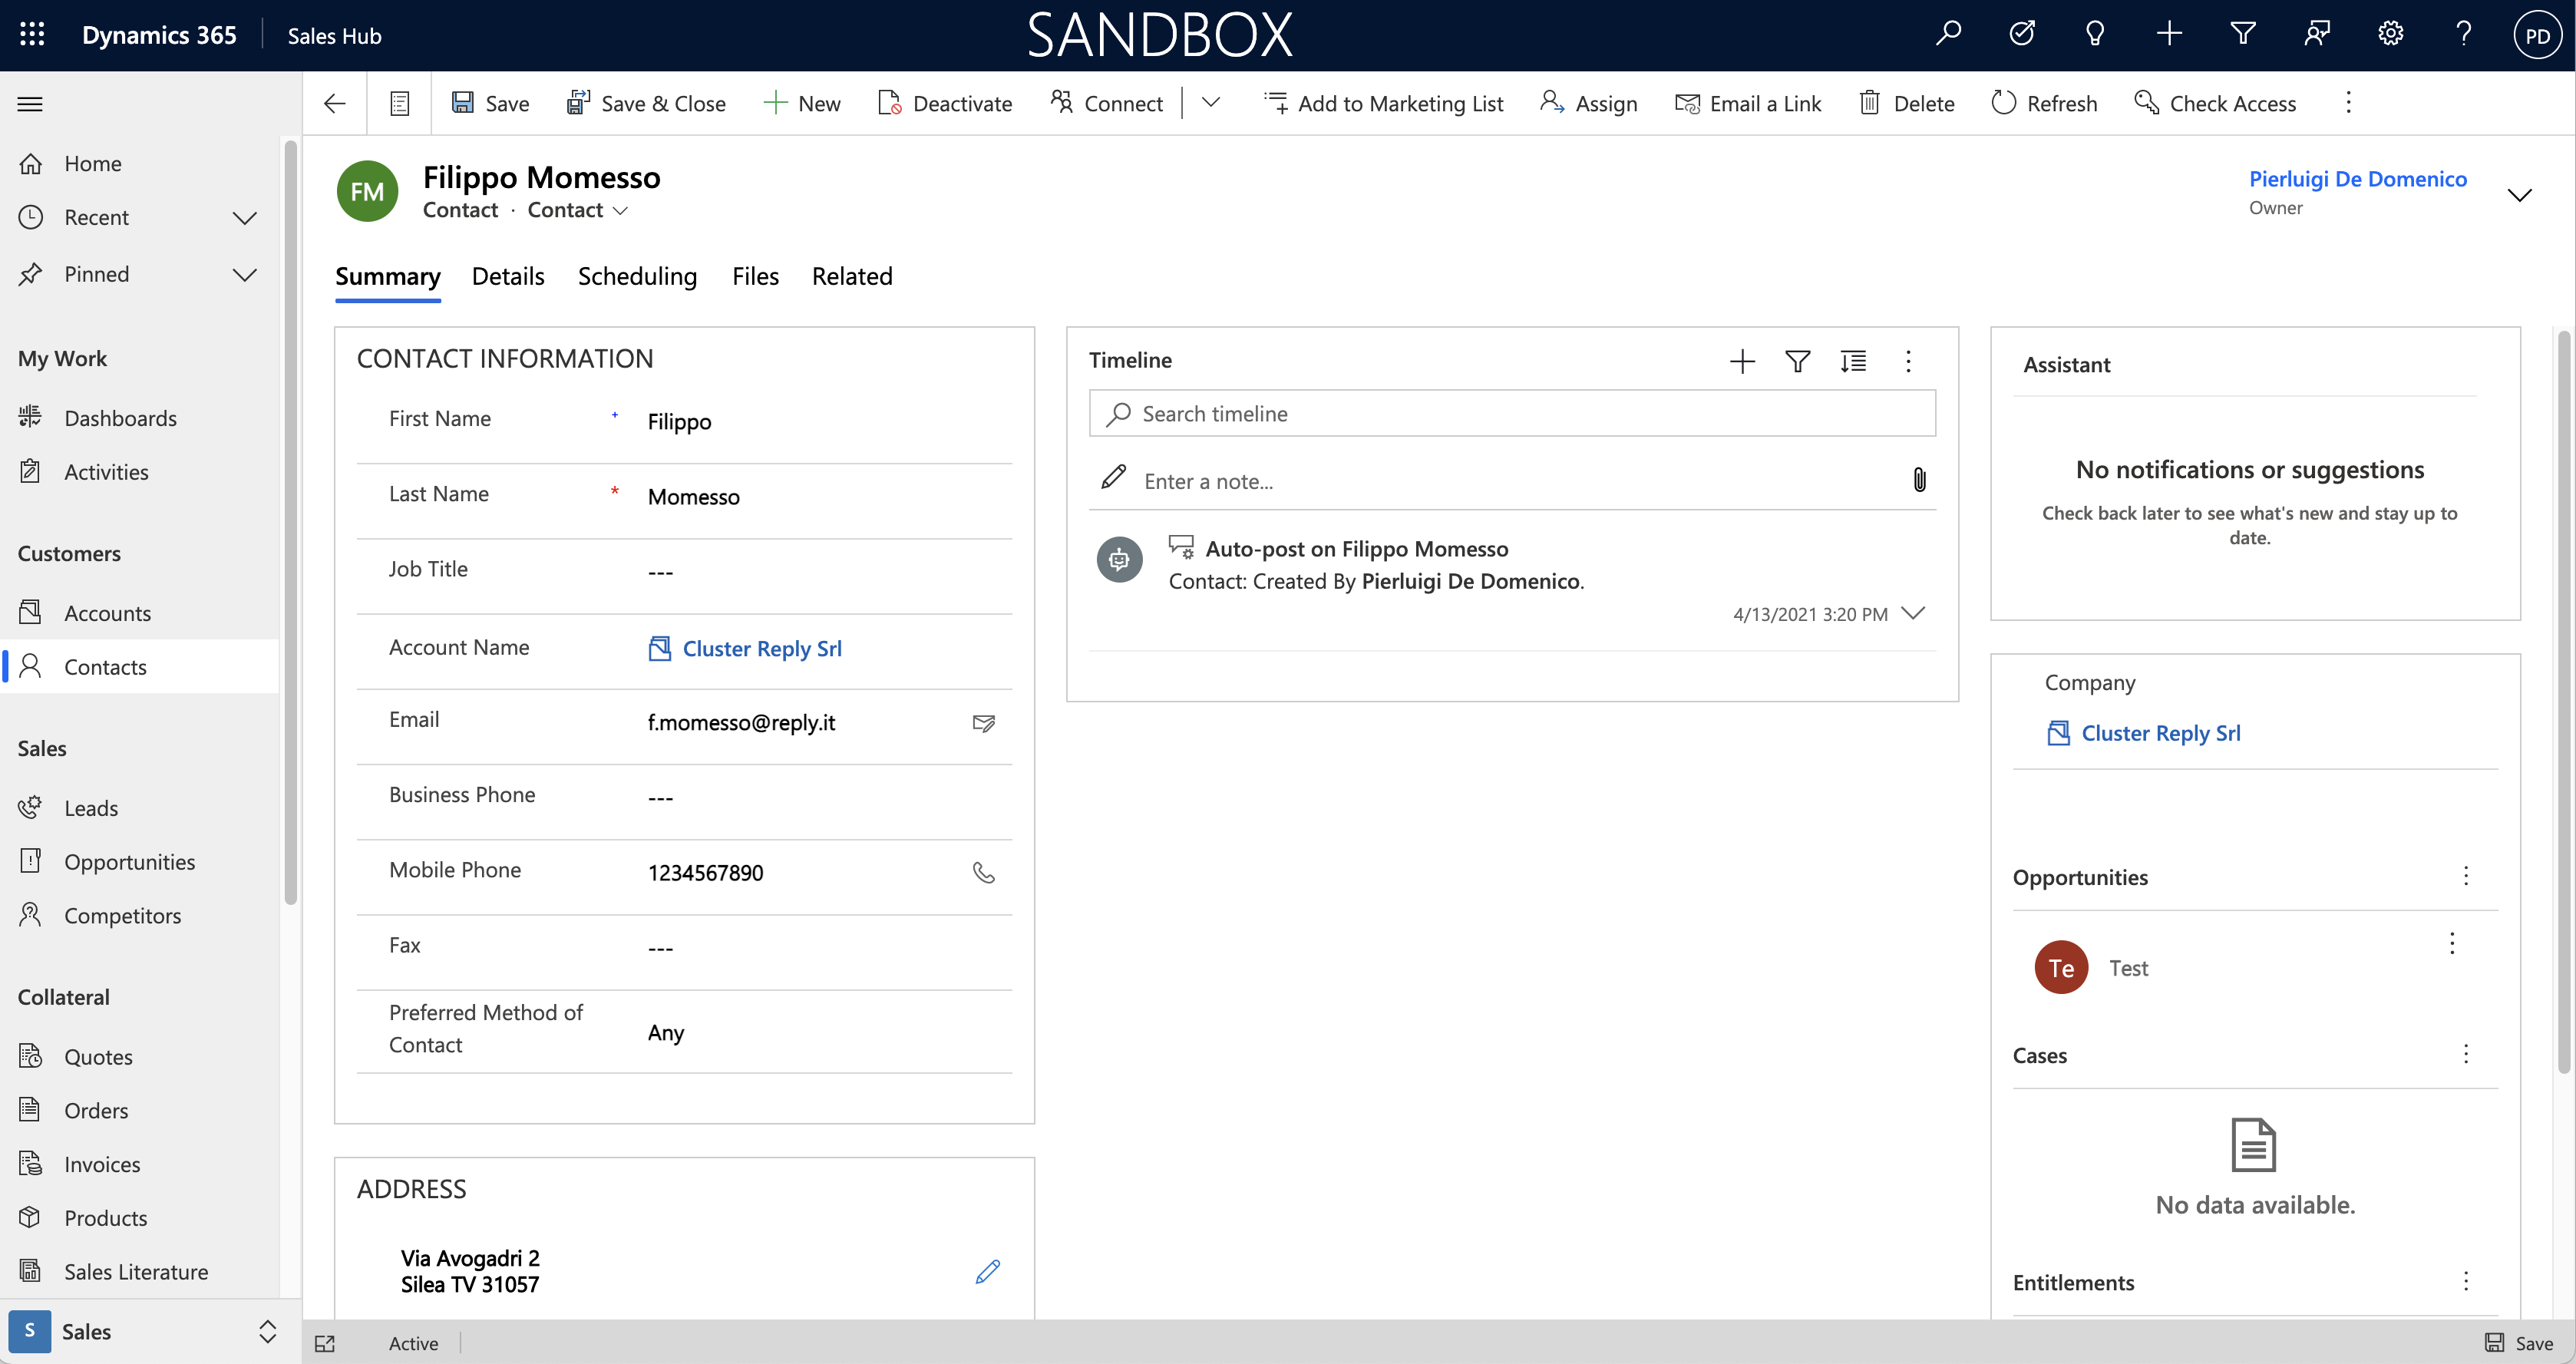
\includegraphics[width=0.7\textwidth]{form-example.png}
  \caption{Esempio di form per la modifica di un record Contact}
  \label{fig:formExample}
\end{figure}

\subsection{Ricerca e Ricerca Avanzata}
Una delle più importanti funzionalità predefinite di Microsoft Dynamics CRM si trova nelle sue capacità di ricerca, le quali forniscono la possibilità di costruire \textit{query} e filtri molto avanzati senza la necessità da parte dell'utente di conoscere linguaggi di programmazione o di querying.

Di default la vista a griglia di ogni entità supporta una funzionalità di Ricerca Veloce mediante una barra di ricerca posizionata nell'interfaccia utente in alto a destra come si può osservare in Figura~\ref{fig:quickSearch}.
\begin{figure}[ht]
  \centering
  
\includegraphics[width=0.7\textwidth]{quick-search.png}
  \caption{Opzioni di ricerca rapida e avanzata.}
  \label{fig:quickSearch}
\end{figure}

Cliccando invece sull'icona cerchiata in rosso in Figura~\ref{fig:quickSearch} si accede alla ricerca avanzata, disponibile in una nuova finestra. La ricerca avanzata del CRM è una delle funzionalità più utili e potenti disponibili di default. In questa finestra, come si vede in Figura~\ref{fig:advancedSearch}, è possibile selezionare l'entità di cui di vogliono cercare i record, applicare filtri e criteri di raggruppamento e salvare i risultati come viste (\textit{views}) personali.
\begin{figure}[ht]
  \centering
  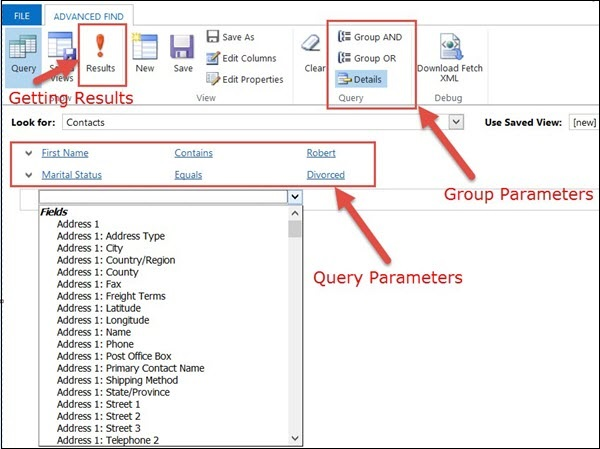
\includegraphics[width=0.7\textwidth]{advanced-search.png}
  \caption{Finestra di ricerca avanzata.}
  \label{fig:advancedSearch}
\end{figure}

\subsection{Web Resources}
 Le \textit{Web Resources} nel CRM sono i file virtuali salvati nel database del CRM e usati per implementare le funzionalità della pagine web del CRM. Questi file possono essere HTML, Javascript, Silverlight o di qualsiasi altro tipo supportato. 
 Nonostante il CRM venga fornito da Microsoft con una serie di funzionalità di base, spesso si rende necessario estendere e personalizzare queste funzionalità per rispettare e implementare i requisiti del progetto in questione. Tali estensioni possono avvenire in genere in due modi:
 \begin{itemize}
   \item \textbf{Estensione lato client} - Usando le Web Resources e il \textit{Form Scripting}.
   \item \textbf{Estensione lato server} - Mediante \textit{Plugin}, \textit{Workflow} e \textit{Web Services}.
 \end{itemize}

Per capire quando può essere necessario l'utilizzo delle Web Resources del CRM prendiamo in considerazione i seguenti esempi: 
\begin{itemize}
  \item Si rende necessario fare ulteriori validazioni lato client sui campi di un form del CRM.
  \item È necessario costruire una o più pagine completamente custom che utilizzino dati provenienti da sistemi esterni al CRM.
  \item Si vogliono applicare modifiche visive o funzionali all'interfaccia grafica standard del CRM.
  \item Si vuole richiamare l'esecuzione di servizi web esterni in seguito ad azioni lato client, senza dover scomodare l'utilizzo di plugin o workflow lato server.
\end{itemize}

L'accesso a una Web Resource può avvenire mediante il suo URL univoco. Dato che le Web Resource vengono salvate nel database del CRM, possono essere caricate come singolo file o come collezione eterogenea di file (HTML, Javascript, ecc.) oppure possono essere create e/o modificate direttamente dal CRM, mediante un pannello apposito. Questo consente inoltre di semplificare i passaggi in caso di migrazione da un ambiente a un altro, come per qualsiasi altra personalizzazione del CRM. In Tabella~\ref{table:webResourceType} vi è un elenco dei principali tipi di web resource supportati.

\begin{table}[ht]
  \centering
  \begin{tabular}{lp{0.6\textwidth}}
    \toprule
      \textbf{Tipo di Web Resource} & \textbf{Esempio} \\ 
    \midrule
      Pagina Web (HTML) & È possibile creare una qualsiasi pagina HTML e inserirla in un form del CRM. \\
      \midrule 
      Fogli di stile (CSS) & Qualsiasi file css che può essere usato insieme ai file HTML. \\ 
      \midrule
      Script (Javascript) & Qualsiasi tipo di codice lato client per manipolare campi, valori, effettuare validazioni, ecc. \\ 
      \midrule
      Dati (XML) & Usati per salvare impostazioni o dati di configurazione in modo statico. \\
      \midrule 
      Immagini (PNG, JPG, GIF, ICO) & Qualsiasi immagine da utilizzare nel CRM.\\ 
      \midrule
      Silverlight (XAP) & Qualsiasi applicazione Microsoft Silverlight da utilizzare nel CRM. \\ 
      \midrule
      Fogli di stile (XSL) & Da usare per trasformare dati XML. \\ 
      \bottomrule
  \end{tabular}
  \caption{Tipi di Web Resource supportati}
  \label{table:webResourceType}
\end{table}

\subsection{Workflow}
I \textit{Workflow} permettono di automatizzare processi di business all'interno del CRM. Possono essere creati utilizzando le funzionalità del CRM oppure mediante lo sviluppo di codice .NET, consigliato nel caso di worflow più complessi. I workflow possono essere eseguiti in background oppure in tempo reale e possono anche richiedere l'input dell'utente.

L'esecuzione di un workflow può essere avviata automaticamente, in base a specifiche condizioni, oppure manualmente dall'utente (ad esempio tramite la pressione di un pulsante o la selezione di un'opzione nel CRM). Internamente i workflow sono implementati utilizzando Windows Workflow Foundation, una tecnologia Microsoft che fornisce un'API, un motore di workflow e un designer per implementare workflow all'interno di applicazioni .NET.

I workflow del CRM possono essere eseguiti in maniera sincrona o asincrona. In genere, si utilizza l'approccio asincrono, facendo eseguire il workflow in background in quanto in questo modo si può limitare l'utilizzo di risorse del sistema.

L'esecuzione di un workflow può avvenire in seguito a specifici eventi definiti dal \textit{Message} del workflow (ovvero il tipo di evento sul quale un Workflow può essere registrato) i quali possono essere creazione, modifica di uno o più valori o eliminazione di un record. Inoltre, un workflow può avere uno \textit{scope} (in italiano "ambito di lavoro") che può essere User, Business Unit, Parent Child Business Unit o Organization. È possibile quindi specificare su quali record potrà essere eseguito il workflow in base all'utente proprietario dei record e del workflow.

Un workflow dunque non è altro che una sequenza di passaggi che vengono eseguiti sul CRM. Possono essere condizionali, di attesa o azioni. I primi due tipi sono auto esplicativi mentre nel terzo si può avere ad esempio la creazione o l'aggiornamento di un record, l'assegnamento di un record a un utente, l'invio di un'email, l'esecuzione di uno step custom programmato in .NET da uno sviluppatore oppure l'interruzione dell'esecuzione del workflow.

\subsection{Plugin}
Un \textit{Plugin} è pezzo di software che si integra con Microsoft Dynamics CRM per modificarne o estenderne il comportamento standard. I plugin si comportano come gestori di eventi (\textit{event handler}) e vengono eseguiti in seguito a un particolare evento nel CRM, specificato in fase di registrazione del plugin. Possono essere scritti in linguaggio C\# oppure Visual Basic e possono essere eseguiti in modalità sincrona o asincrona.

Alcuni esempi di scenari in cui un Plugin può essere utilizzato sono:
\begin{itemize}
  \item È necessario eseguire delle operazioni in modo automatico in seguito all'aggiornamento di alcuni determinati campi di un record, oppure aggiornare altri record collegati in seguito alla modifica o alla creazione di un record nel CRM.
  \item Si vuole chiamare un servizio web esterno in seguito a un evento come la creazione o l'aggiornamento di un record.
  \item È necessario compilare in modo dinamico i valori di alcuni campi di un record.
  \item Si vuole automatizzare dei processi come l'invio di email in seguito a specifici eventi nel CRM.
\end{itemize}

La pipeline di un plugin è divisa in molteplici fasi su cui può essere registrata la logica del plugin. La fase (in inglese \textit{stage}) indica in quale punto del ciclo di esecuzione del plugin deve essere eseguito il codice. In Tabella~\ref{table:pluginStages} si possono consultare le fasi per cui è possibile registrare un plugin.  

\begin{figure}[ht]
  \centering
  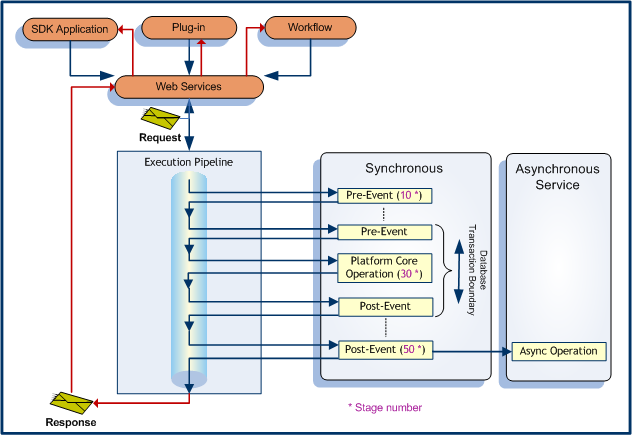
\includegraphics[width=0.7\textwidth]{plugin-pipeline.png}
  \caption{Pipeline di un Plugin}
  \label{fig:pluginPipeline}
\end{figure}

\begin{table}[ht!]
  \centering
  \begin{tabular}{p{0.15\textwidth}lp{0.55\textwidth}}
    \toprule
      \textbf{Evento} & \textbf{Nome della fase} & \textbf{Descrizione} \\
    \midrule
      Pre-Event & Pre-validation &  Fase della pipeline per i plugin che devono essere eseguiti prima della MainOperation. I plugin registrati in questa fase possono essere eseguiti all'\textbf{esterno} della transazione del database. \\
    \midrule
      Pre-Event & Pre-operation & Fase della pipeline per i plugin che devono essere eseguiti prima della MainOperation. I plugin registrati in questa fase sono eseguiti all'\textbf{interno} della transazione del database. \\
    \midrule
      Platform Core Operation & MainOperation &  L'operazione principale eseguita dal sistema, come creazione, aggiornamento, eliminazione di un record. Nessun plugin può essere registrato per questa fase. \\
    \midrule
      PostEvent & Post-operation &  Fase della pipeline per i plugin che devono essere eseguiti dopo della MainOperation. I plugin registrati in questa fase sono eseguiti all'\textbf{interno} della transazione del database. \\
    \bottomrule
  \end{tabular}
  \caption{Fasi del ciclo di esecuzione di un Plugin}
  \label{table:pluginStages}
\end{table}

Ogni volta che il CRM invoca un evento, come ad esempio il salvataggio di un record, viene eseguita una sequenza di azioni.
Per prima cosa l'evento innesca la chiamata al CRM Organization Web Service e l'esecuzione viene fatta passare attraverso le fasi della pipeline. Internamente le informazioni vengono trasmesse mediante un messaggio di tipo OrganizationRequest il quale viene intercettato dai plugin di tipo Pre-Event che possono modificarne le informazioni prima che venga passato alla Platform Core Operation. Dopodiché il messaggio viene trasformato in un OrganizationResponse che viene intercettato dai plugin Post-Operation i quali possono modificarne le informazioni prima.
Infine, l'esecuzione viene ritornata all'applicazione che ha invocato l'evento.

Il campo \textit{Message} specifica, come nel caso dei Workflow, il tipo di evento su cui il plugin è registrato. Per esempio, un plugin può essere registrato su un Create Message di un'entità Contact. In questo caso il codice del plugin verrebbe eseguito ogni qual volta un record Contact viene creato. Per le entità di default del CRM sono supportati più di 100 message diversi, mentre per le entità custom la scelta è più limitata.

\subsubsection{Differenze tra Workflow e Plugin}
Sia i Workflow che i Plugin possono essere utilizzati per estendere e le funzionalità del CRM. In molti casi i due approcci sono intercambiabili e possono essere utilizzati uno al posto dell'altro senza nessun problema. 
Tuttavia, la documentazione ufficiale Microsoft~\cite{PluginVSWorkflow} suggerisce alcune linee guida riportate in Tabella~\ref{table:pluginVsWorkflow}. Inoltre, i colleghi più esperti mi hanno spiegato che in generale preferiscono usare i plugin in caso di logica sincrona oppure molto complessa, mentre i workflow per la logica asincrona o per processi semplici e da eseguire in seguito a una richiesta dell'utente, come ad esempio l'invio automatico di email.

\begin{table}[ht]
  \centering
  \begin{tabular}{p{0.14\textwidth}p{0.39\textwidth}p{0.39\textwidth}}
    \toprule
      \textbf{Criterio} & \textbf{Plugin} & \textbf{Workflow} \\
    \midrule
    Eseguito prima o dopo la Core Platform Operation & Viene eseguito immediatamente prima o dopo la core operation (sincrono). Può essere messo in coda ed eseguito dopo la core operation (asincrono) & Viene messo in coda ed eseguito dopo la core operation \\
    \midrule
    Impatto sulle perfomance del CRM & Plugin sincroni possono aumentare i tempi di risposta del CRM in quanto fanno parte dei processi della piattaforma. Un plugin mal implementato può bloccare il CRM & L'impatto negativo sui tempi di risposta del CRM è minimo. \\
    \midrule
    Restrizioni di sicurezza & Per registrare un plugin è necessario un utente con i privilegi di System Admin o System Customizer che sia membro del Deployment Administrator group & Gli utenti possono creare workflow in modo interattivo all'interno dell'interfaccia web. Tuttavia, per poter registrare un workflow è necessario avere gli stessi privilegi di sicurezza richiesti per i plugin. \\
    \midrule
    Migliore per operazioni che richiedono molto o poco tempo & I plugin ad esecuzione sincrona andrebbero usati per processi brevi mentre i plugin asincroni per operazioni più intensive. & Indifferentemente per processi brevi o lunghi. \\
    \midrule
    Persistenza del processo e dei dati & I plugin vengono eseguiti fino al completamento & I workflow possono essere messi in pausa, posposti, cancellati e ripresi mediante chiamate all'SDK o dall'utente mediante l'interfaccia web del CRM. Lo stato di un Workflow viene salvato automaticamente prima di essere messo in pausa o posposto. \\
    \bottomrule
  \end{tabular}
  \caption{Come scegliere se utilizzare un Plugin o un Workflow}
  \label{table:pluginVsWorkflow}
\end{table}

\subsection{Soluzioni}
Le soluzioni sono il modo con cui è possibile firmare, impacchettare e manutenere le unità software che estendono il CRM~\cite{Solutions}. Qualsiasi customizzazione, estensione, o configurazione può essere impacchettata, organizzata e distribuita usando le soluzioni. Una soluzione può essere esportata come file .zip e importata in seguito in un'altra istanza di Dynamics 365. 
\subsubsection{Tipi di soluzioni}
Esistono tre tipi di soluzioni: la Default System Solution, le soluzioni Managed e le soluzioni Unmanaged.

La prima contiene tutti i componenti definiti di default in Microsoft Dynamics CRM senza alcuna customizzazione. Questi componenti possono essere modificati e le versioni modificate possono essere inserite in soluzioni di tipo Managed o Unmanaged.

Una soluzione Managed è una soluzione che si intende distribuire e installare nel CRM del cliente. In particolare può essere installata sulla soluzione di default o su altre soluzioni Managed. Su una soluzione di questo tipo non è possibile quindi aggiungere o rimuovere componenti, è tuttavia permessa la modifica dei componenti presenti.

Una soluzione Unmanaged è una soluzione da considerarsi ancora in fase di sviluppo e che non si intende distribuire. In una soluzione Unmanaged è possibile aggiungere, rimuovere, modificare ed eliminare componenti. Ogni nuova soluzione inoltre è impostata di default come di tipo Unmanaged.

\section{Microsoft Power Automate}
Microsoft Power Automate, in precedenza conosciuto come Microsoft Flow, è un servizio online per la creazione di flussi di lavoro \textit{low-code/no-code} in grado di automatizzare operazioni su diverse app e servizi, sia sviluppati da Microsoft che non.
È possibile connettersi infatti a più di 220 servizi e gestire i dati sia in cloud che in locale come ad esempio con SharePoint o Microsoft SQL Server. La lista di connettori ad app e servizi disponibili inoltre, è in continua crescita in quanto Microsoft lavora a stretto contatto con i vari partner per estendere le possibilità di Power Automate.

I due principali tipi di flussi di lavoro supportati da Power Automate sono i flussi cloud e i flussi desktop.
\paragraph{Flussi Cloud} Si dividono in tre tipologie:
\begin{itemize}
  \item Flussi automatizzati - Permettono di creare un'automazione che viene attivata da un evento come l'arrivo di un email da una persona specifica. 
  \item Flussi istantanei - Permettono di avviare un'automazione facendo click su un pulsante. È possibile automatizzare le azioni ripetitive come ad esempio l'invio di un promemoria su Microsoft Teams
  \item Flussi pianificati - Permettono di pianificare un'automazione ad una specifica ora come ad esempio il caricamento giornaliero di dati in SharePoint o in un database
\end{itemize}

\paragraph{Flussi Desktop} Vengono utilizzati per automatizzare attività ripetitive sul Web o sul desktop. È possibile ad esempio creare flussi per organizzare documenti mediante azioni su file e cartelle, estrarre dati da siti web e archiviarli su file Excel, inserire fatture in software gestionali e molto altro.

\begin{figure}[ht!]
  \centering
  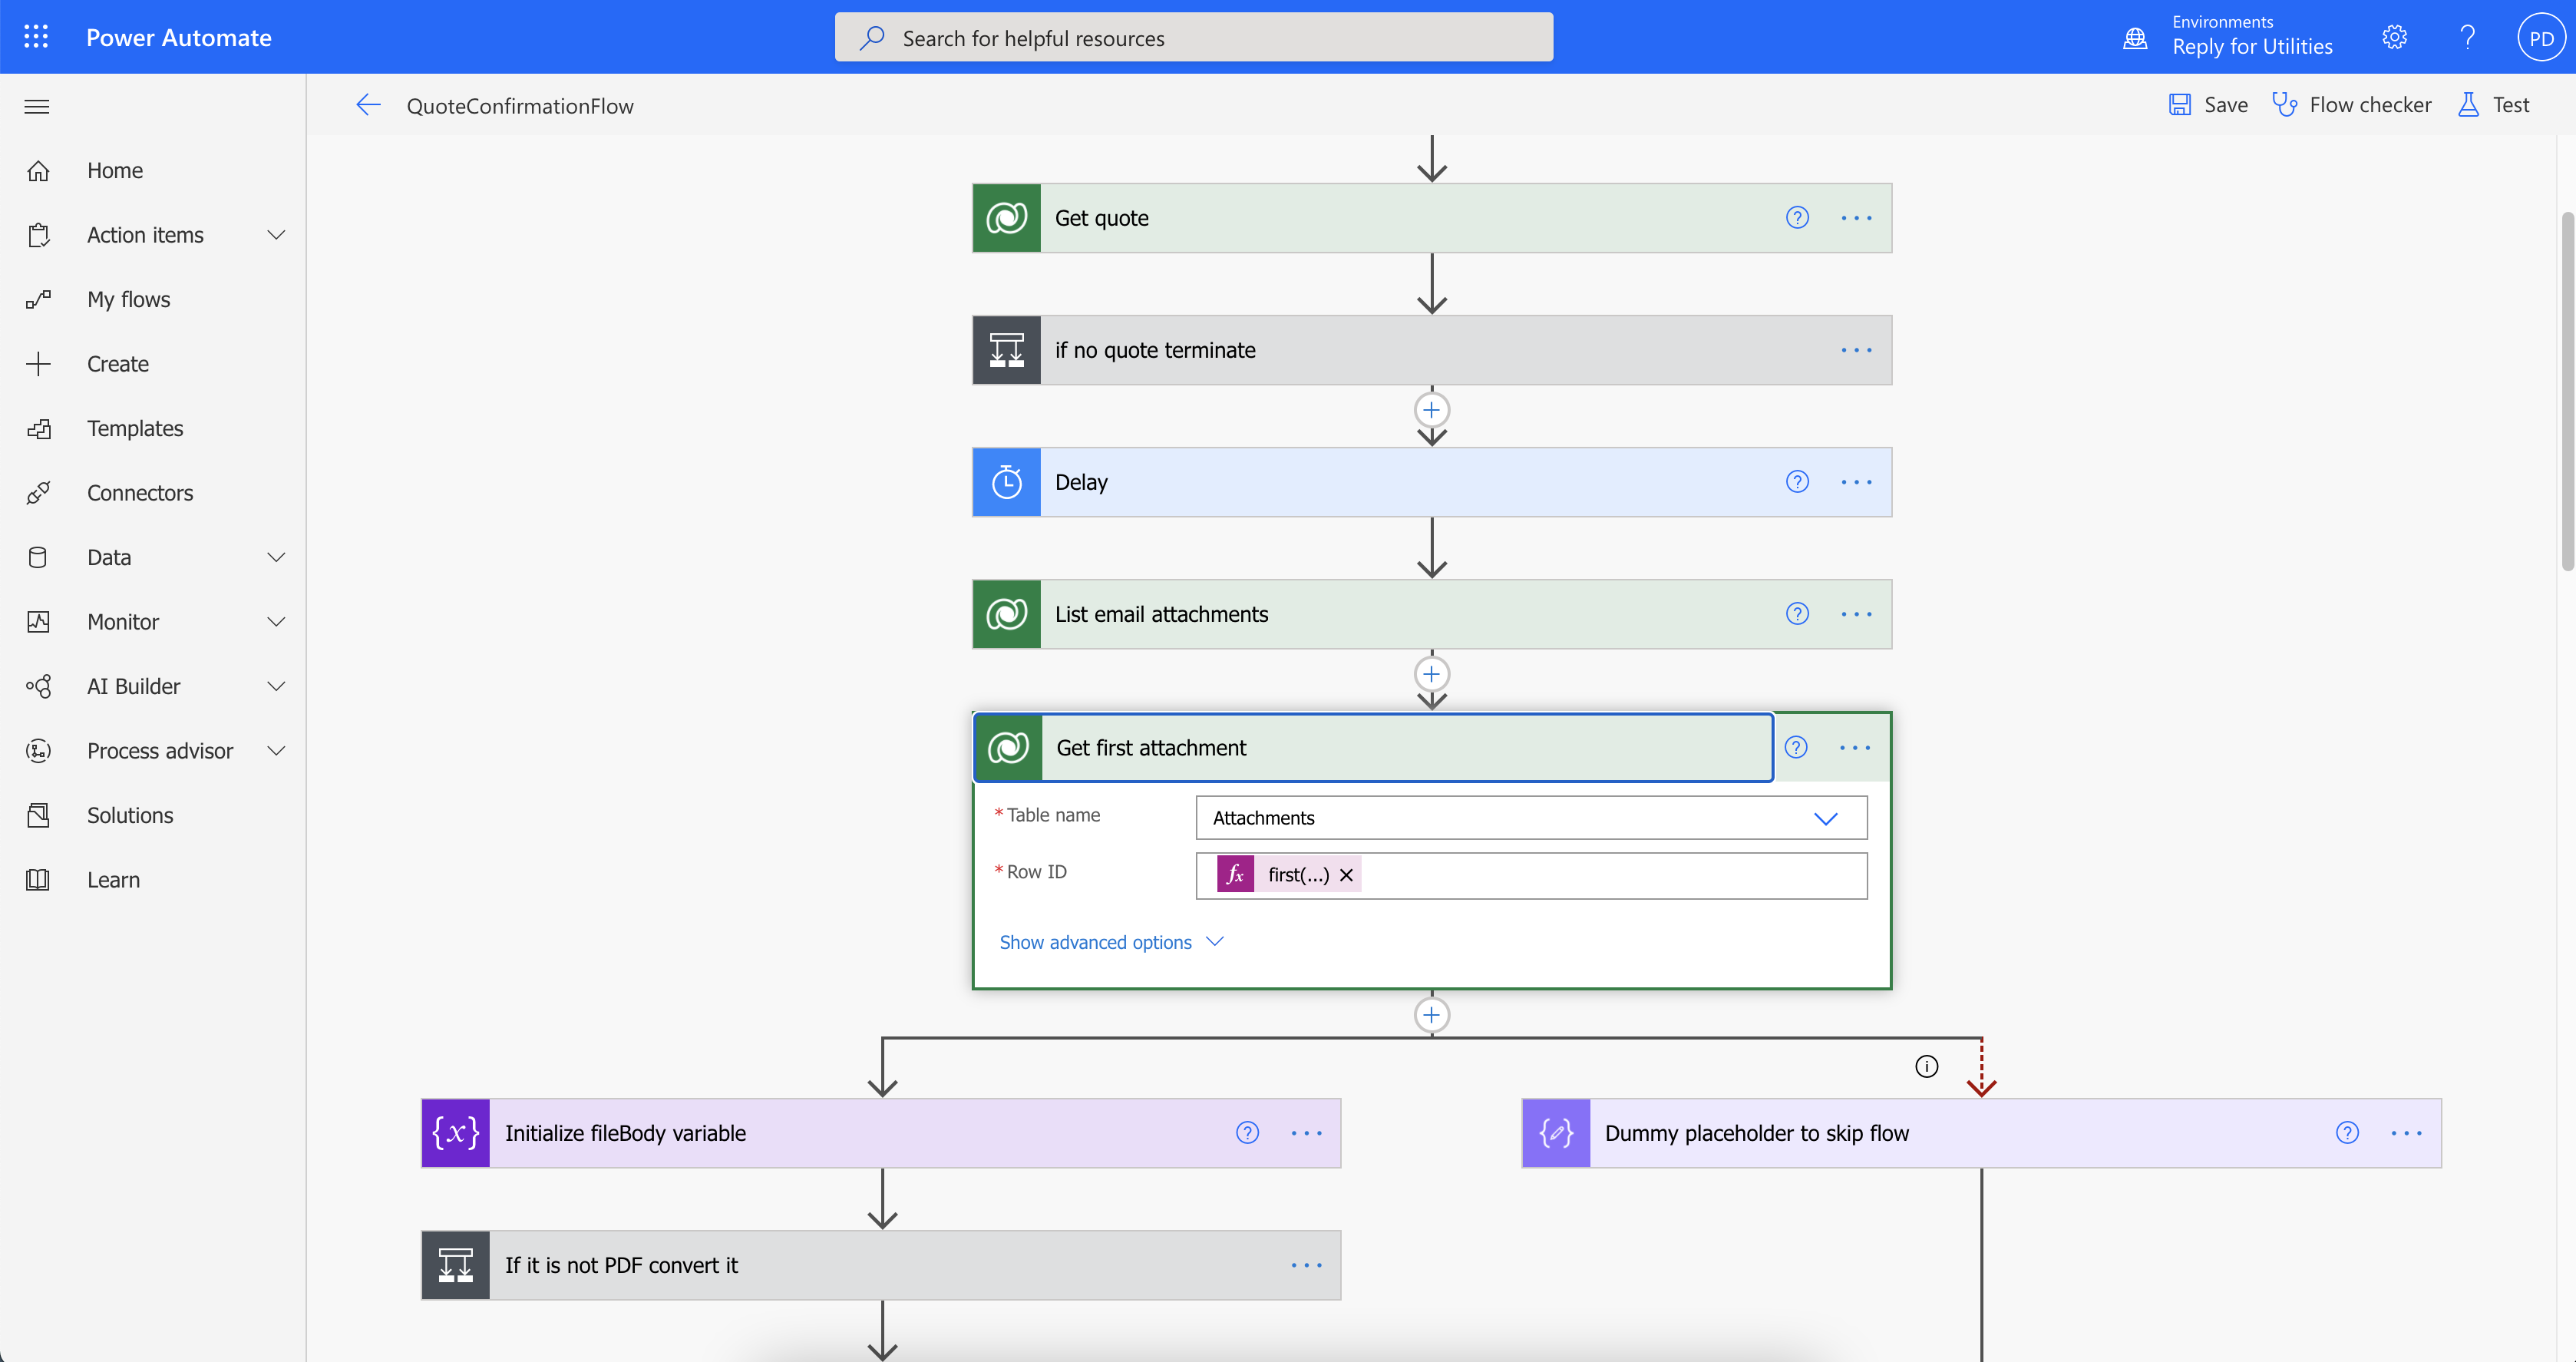
\includegraphics[width=0.9\textwidth]{flow-example.png}
  \caption{Esempio di un flusso Power Automate}
  \label{fig:flowExample}
\end{figure}

\subsection{Flussi Cloud}
In Microsoft Power Automate un flusso è rappresentato mediante un diagramma a blocchi come si può vedere in Figura~\ref{fig:flowExample}. Ogni flusso inizia sempre con un blocco di tipo \textit{trigger}, il quale permette di avviare l'esecuzione del flusso in seguito al verificarsi di un evento specificato. La maggior parte dei connettori disponibili offre diversi trigger predefiniti da utilizzare per avviare i flussi. Tutti gli altri blocchi utilizzabili sono blocchi di tipo \textit{action} e permettono di eseguire operazioni come la creazione di record nel CRM, la chiamata ad API esterne, l'invio di email e altro, a seconda di ciò che viene reso disponibile dai vari connettori.

Un connettore non è altro che un proxy o un wrapper intorno a un'API che consente al servizio sottostante di comunicare con Microsoft Power Automate. Consente agli utenti di connettere i loro account e sfruttare un set di trigger e azioni predefiniti per sviluppare i flussi di lavoro. Microsoft mette a disposizione numerosi connettori (gratuiti e a pagamento) già pronti per essere utilizzati ed è possibile inoltre per gli sviluppatori creare dei connettori custom per poter integrare il proprio servizio web o API nell'ecosistema Power Automate.

\begin{figure}[ht!]
  \centering
  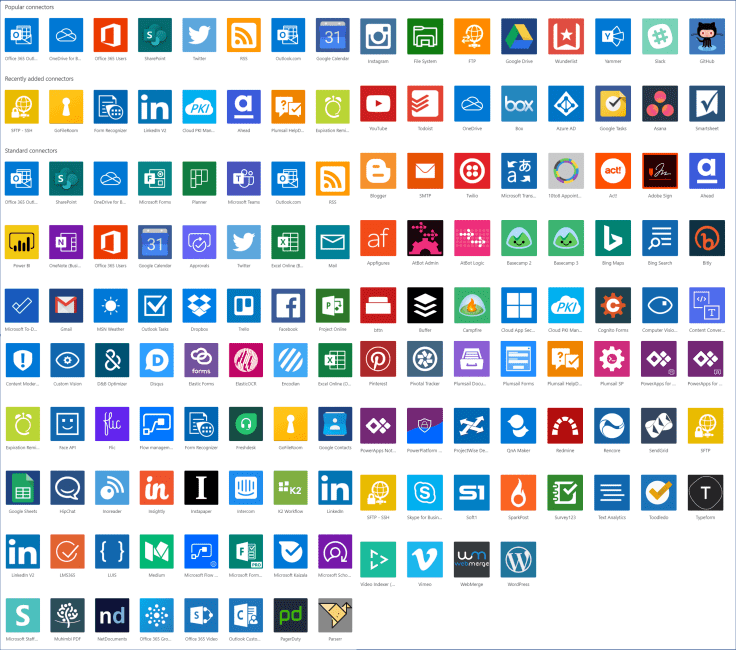
\includegraphics[width=0.6\textwidth]{connectors.png}
  \caption{Elenco dei connettori gratuiti di Power Automate.}
  \label{fig:connectors}
\end{figure}

\subsubsection{Trigger e Action}
Attraverso l'interfaccia grafica è possibile creare blocchi trigger e action, ai quali si possono passare dati o espressioni in maniera molto semplice e intuitiva come in Figura~\ref{fig:actionExample} nella quale è visibile una action per la creazione di un file su dropbox che utilizza i dati di un tweet restituiti da un trigger. Attraverso il pannello laterale \textit{Dynamic Content} si possono inserire i valori dinamici ritornati da action o trigger precedenti. È possibile inserire espressioni in linguaggio OData all'interno dei campi di testo oppure espressioni più complesse  in linguaggio \textit{Workflow Definition Language} mediante il pannello laterale \textit{Expression}\cite{WorkflowDefinitioLanguage}.
\begin{figure}[ht]
  \centering
  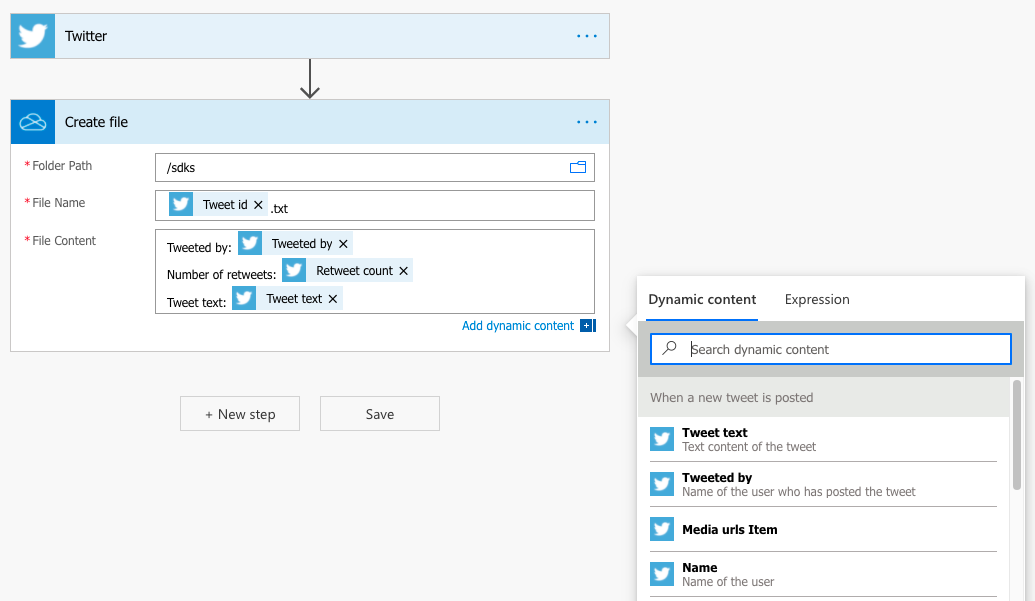
\includegraphics[width=0.9\textwidth]{action-example.png}
  \caption{Esempio di blocco di tipo action.}
  \label{fig:actionExample}
\end{figure}

Dietro a questa semplice e intuitiva interfaccia grafica non si nasconde altro che un oggetto JSON definito rispettando le specifiche del linguaggio sopracitato. Di seguito il listato corrispondente all'action usata come esempio.

\lstinputlisting[language=json]{chapters/02/onedrive-action.json}

 \section{Microsoft AI Builder}
Microsoft AI Builder è una funzionalità di Power Platform che permette l'utilizzo di modelli di intelligenza artificiale per ottimizzare i processi aziendali. Essendo parte di Power Automate, anche AI Builder sposa la filosofia low-code/no-code permettendo all'utente di utilizzare modelli di machine learning preconfezionati senza la necessità di competenze di programmazione o \textit{data science}.
Essendo una tecnologia completamente closed-source Microsoft non ha reso disponibili molte informazioni sull'architettura e il funzionamento dietro le quinte di AI Builder. L'unica informazione disponibile è che viene sfruttata la stessa tecnologia del pacchetto di servizi Microsoft Azure AI, anch'essa closed-source.

In AI Builder è possibile scegliere tra diversi tipi di modelli a seconda dello scenario di utilizzo. Questi si dividono in modelli predefiniti e modelli personalizzati.
La differenza tra le due tipologie si trova nel fatto che nel primo caso il modello è fornito pronto all'uso, mentre nel secondo è necessario creare, sottoporre a training e pubblicare per l'uso il modello in questione.

\begin{multicols}{2}
  Modelli predefiniti:
    \begin{itemize}
      \item Estrazione di parole chiave
      \item Rilevamento lingua
      \item Analisi del sentimento
      \item Traduzione testo
      \item Lettore di biglietti da visita
      \item Riconoscimento del testo
      \item Elaborazione ricevute
    \end{itemize}
\columnbreak
  Modelli personalizzati:
    \begin{itemize}
      \item Classificazione categoria
      \item Estrazione di entità
      \item Stima
      \item Elaborazione moduli
      \item Rilevamento oggetti
    \end{itemize}
\end{multicols}

\begin{figure}[ht!]
  \centering
  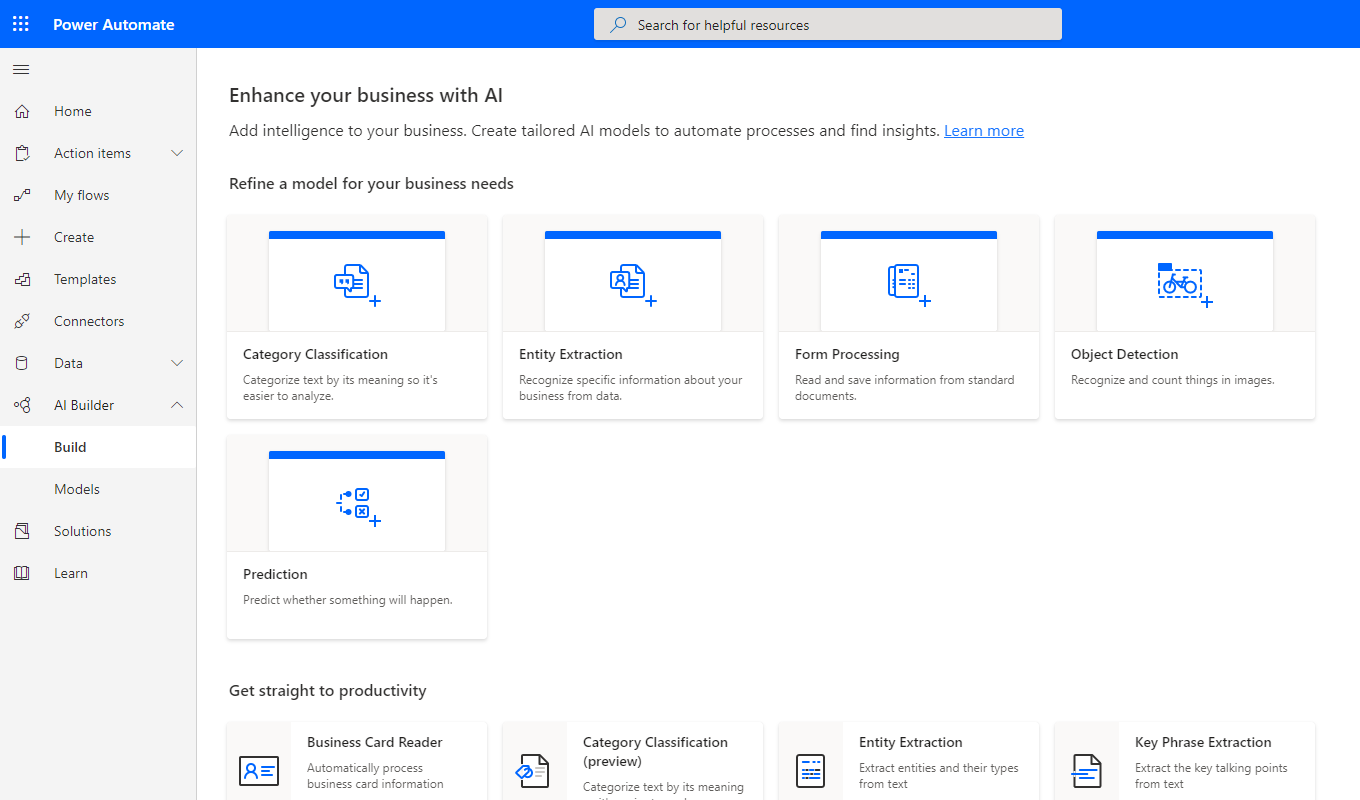
\includegraphics[width=0.8\textwidth]{ai-builder-home.png}
  \caption{Schermata home di AI Builder.}
  \label{fig:aiBuilderHome}
\end{figure}

\subsection{Creazione di un modello personalizzato}
Nel caso di modelli personalizzati in fase di creazione di un modello è necessario fornire un dataset di training. Essendo una feature low-code/no-code i passaggi necessari sono abbastanza semplici. Per fornire il dataset di training si hanno due possibilità a seconda del tipo di dati che il modello in questione prende come input: testo o immagini/documenti. Se il modello effettua analisi di testo il dataset di training dovrà essere fornito utilizzando una tabella Dataverse, un altro servizio Microsoft che permette di archiviare e gestire dati utilizzati nelle applicazioni Microsoft. Questa tabella dovrà contenere i dati di training secondo le specifiche definite per il singolo modello. In altre parole, modelli diversi richiedono dati diversi, etichettati in modo diverso. 
Se il modello lavora su dati come documenti o immagini, invece, si dovrà seguire la procedura guidata all'interno di AI Builder, che permetterà di caricare ed etichettare i documenti su cui fare il training. 

Una volta terminato il training del modello è possibile testarlo, con altri dati non etichettati e valutarne le performance. Dopodiché il modello è pronto per essere pubblicato ed utilizzato in Microsoft Power Automate. Esiste infatti un connettore apposito per AI Builder.

\subsubsection{Esempio: modello di elaborazione moduli}
Il modello di elaborazione moduli fornito da AI Builder consente di leggere e salvare informazioni da documenti standard come fatture o documenti fiscali. Automatizzando questo processo è possibile risparmiare molto tempo evitando, ad esempio, che l'utente debba passare ore a trascrivere a mano fatture all'interno di un gestionale.

Il modello, tuttavia, presenta ancora alcune limitazioni, come ad esempio il formato del file (PDF, JPG, PNG), il numero di pagine  e la dimensione del documento (non più di 500 pagine per i PDF e 50 MB) e il supporto al solo alfabeto latino.
Tra le limitazioni più importanti, inoltre, vi è il mancato supporto al riconoscimento di caselle di controllo, pulsanti di opzione e firme. Queste ultime tre limitazioni in particolare sono state un problema in fase di sviluppo dei progetti.

Per creare il modello personalizzato di elaborazione dei moduli è necessario per prima cosa specificare i nomi dei campi e delle tabelle che dovranno essere estratti dal documento.
In seguito, si dovranno caricare i file su cui avverrà il training del modello. AI Builder a questo punto analizzerà i documenti caricati in modo da rilevare la presenza di campi testuali e tabelle.
L'utente dovrà  selezionare manualmente i campi che si vogliono riconoscere e contrassegnarli con l'etichetta corrispondente come in Figura~\ref{fig:aiBuilderFields}; allo stesso modo è possibile contrassegnare tabelle come in Figura~\ref{fig:aiBuilderTables}. Non sono supportate le tabelle estese su più pagine, pertanto è necessario definirle come tabelle separate durante il primo passaggio della procedura.

Terminato il passaggio di etichettatura di campi e tabelle sui documenti di training, AI Builder procede con il training del modello.

\begin{figure}[ht]
  \centering
  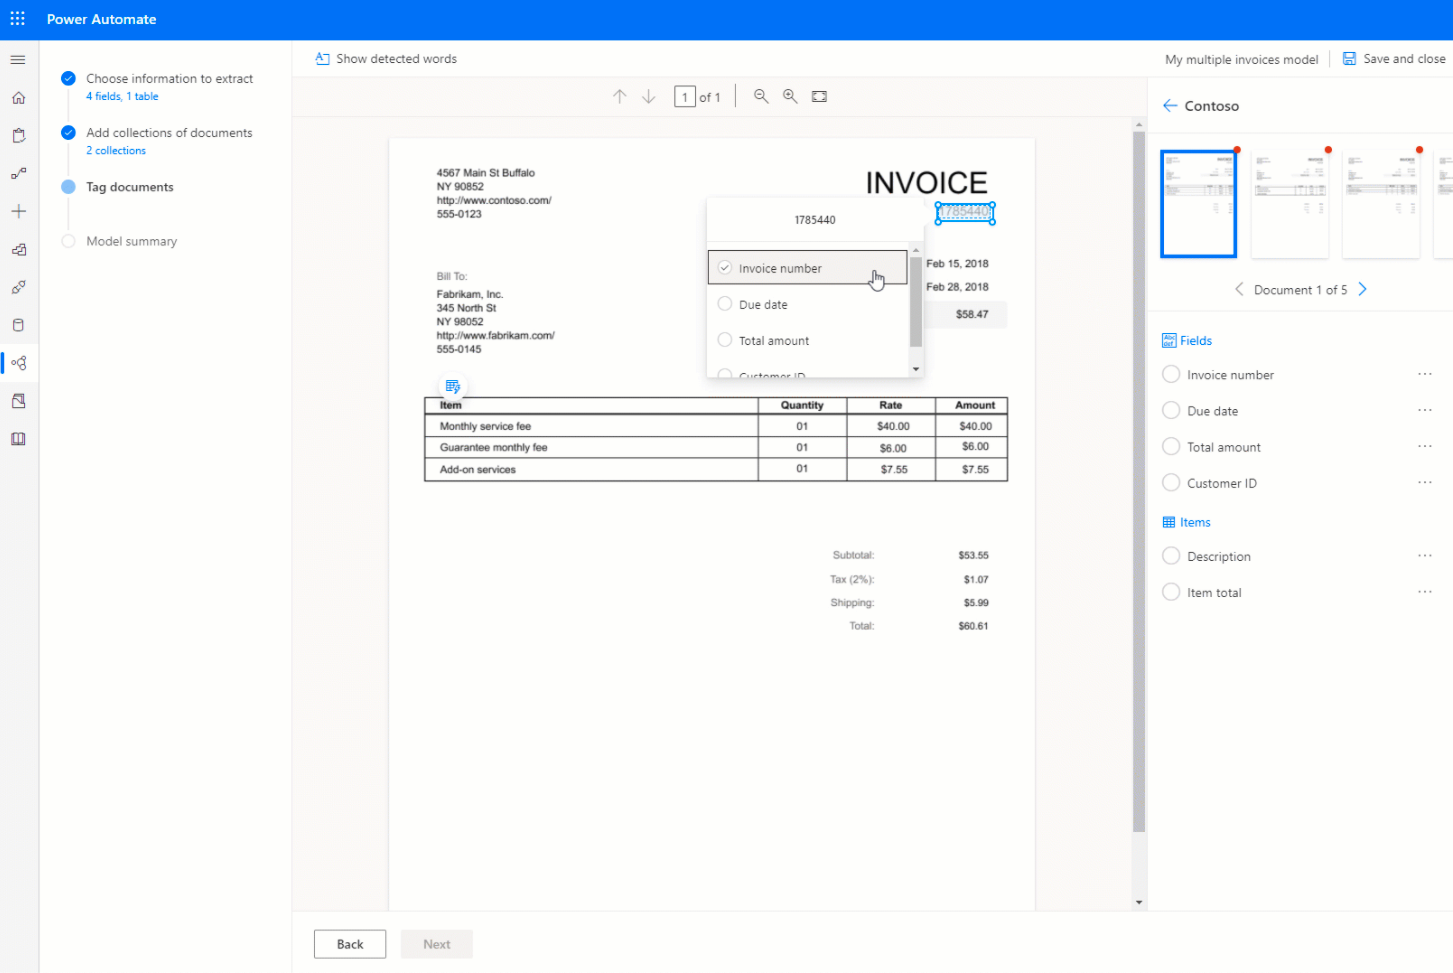
\includegraphics[width=0.9\textwidth]{ai-builder-fields.png}
  \caption{Etichettatura di campi testuali in AI Builder.}
  \label{fig:aiBuilderFields}
\end{figure}

Al termine del training è possibile effettuare un test rapido sulle performance del modello caricando manualmente un documento. In seguito all'analisi, verranno mostrati i campi ed eventuali tabelle riconosciute e una percentuale di \textit{confidence} per ciascun campo. Questo dato indica quanto il modello ritiene di essere stato preciso nel riconoscimento di quel valore. In Figura~\ref{fig:aiBuilderTest} un esempio.
Dopodiché per utilizzare un modello all'interno di app e servizi Microsoft è necessario pubblicarlo mediante l'apposito pulsante.

\begin{figure}[ht]
  \centering
  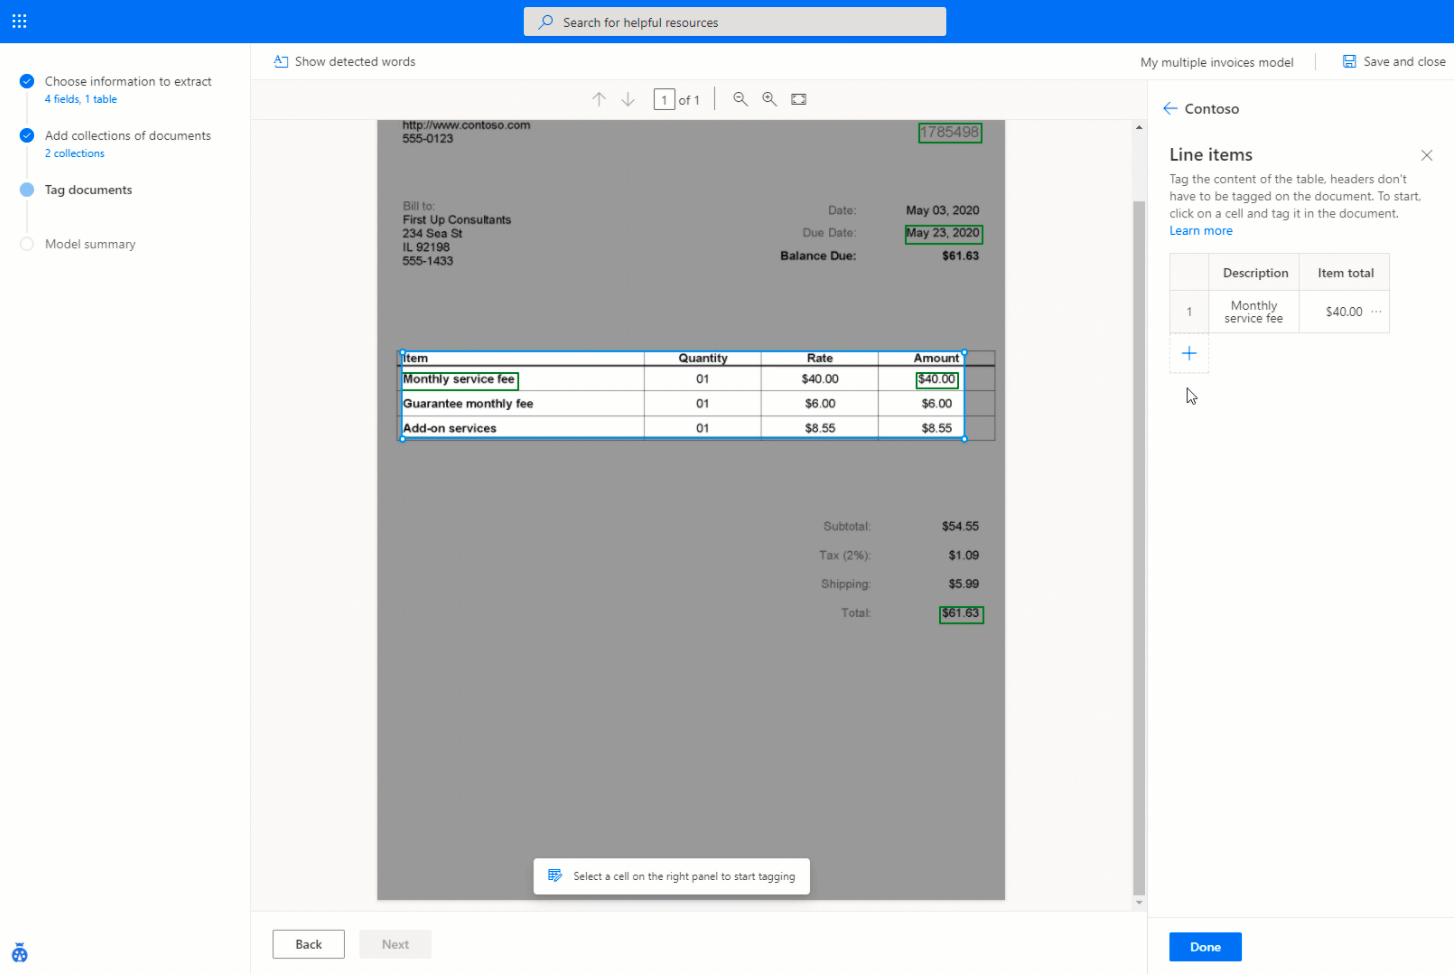
\includegraphics[width=0.9\textwidth]{ai-builder-tables.png}
  \caption{Etichettatura di tabelle in AI Builder.}
  \label{fig:aiBuilderTables}
\end{figure}

\begin{figure}[ht!]
  \centering
  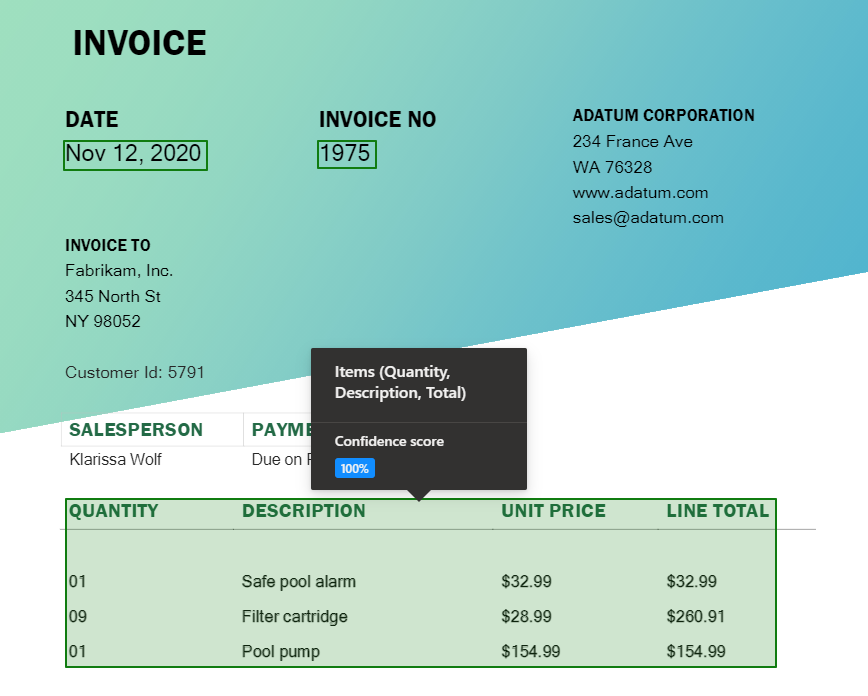
\includegraphics[width=0.8\textwidth]{ai-builder-test.png}
  \caption{Esempio dell'esito del test rapido su un documento.}
  \label{fig:aiBuilderTest}
\end{figure}

\subsubsection{Utilizzo in Power Automate}
Per utilizzare un modello AI Builder in un flusso Power Automate è sufficiente utilizzare l'action  del connettore AI Builder corrispondente al tipo di modello necessario. Per utilizzare un modello di elaborazione dei moduli, ad esempio, bisogna utilizzare la action \textit{Process and save information from forms} e selezionare il modello pubblicato, il tipo di documento e passare il file stesso come contenuto dinamico. Nell'esempio in Figura~\ref{fig:flowAIBuilder} il documento viene recuperato da un trigger manuale che richiede l'inserimento di un file da parte dell'utente. Nulla vieta tuttavia che il documento da analizzare possa essere l'allegato di un'email oppure un file in Onedrive o Sharepoint. Sarà necessario semplicemente utilizzare una action del relativo connettore per recuperare il file desiderato.

Come output viene ritornato un oggetto JSON contenente dati diversi a seconda del tipo di modello utilizzato. Nel caso di esempio per ogni campo vengono ritornati, il valore corrispondente, il punteggio di confidence, le coordinate del riquadro che racchiude il valore, il numero di pagina in cui si trova il valore e altri dati. In appendice è disponibile un esempio di oggetto JSON restituito.
I dati contenuti in questo oggetto inoltre vengono interpretati da Power Automate e resi disponibili come contenuto dinamico per essere utilizzati nel flusso da altre action.

\begin{figure}[ht]
  \centering
  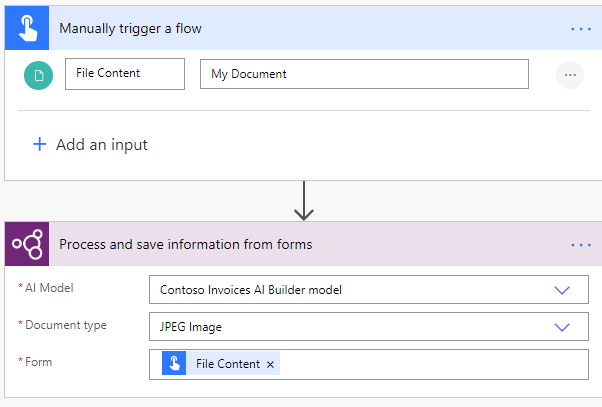
\includegraphics[width=0.7\textwidth]{flow-ai-builder.png}
  \caption{Esempio di utilizzo di una action AI Builder in un flusso Power Automate.}
  \label{fig:flowAIBuilder}
\end{figure}

\subsubsection{Criticità di AI Builder}
Nonostante AI Builder sia uno strumento molto potente per gli utilizzi per cui è proposto, risulta anche molto limitante. Prendendo ad esempio il modello di elaborazione di documenti, che è quello con cui ho avuto più a che fare durante i due progetti, si ottengono risultati positivi solo quando i documenti analizzati sono tra loro identici nella struttura a quelli utilizzati per il training. Le uniche differenze infatti devono trovarsi nei dati contenuti; qualora posizionamento, font e dimensione del testo differiscano, il modello fallisce. Microsoft tuttavia non menziona in nessun modo questo dettaglio nella documentazione.

Inoltre, avendo potuto lavorare con le varie tecniche di machine learning durante il corso \textit{Introduction to Machine Learning}, mi sono trovato impossibilitato a utilizzare le metodologie apprese, in particolare riguardo la validazione e il testing, in quanto AI Builder non fornisce alcun modo per poter effettuare testing su larga scala e quindi raccogliere dati e analizzarli. In sostanza bisogna fidarsi dello strumento e credo che in ambito business non sia una buona pratica. Chiaramente essendo un prodotto mirato a una classe di utenti non esperta credo che il compromesso sia comunque buono.







      \chapter{Progetti sviluppati}
\label{cha:progetti}

      %\graphicspath{{./chapters/04/assets/}}
\chapter{Secondo Progetto}
Il secondo progetto assegnatomi durante il periodo di tirocinio mi ha permesso di approfondire ancora di più le tecnologie trattate nel Capitolo~\ref{cha:analisiTecnologie} e di utilizzare le competenze di programmazione apprese durante il percorso di Laurea, sviluppando dei Plugin in linguaggio C\#. 

La motivazione che ha spinto il supervisore aziendale ad affidarmi questo progetto risiede nel fatto che l'azienda necessitava di una \textit{demo proof-of-concept} da utilizzare come esempio delle possibilità di customizzazione del CRM per i potenziali clienti. Il progetto sviluppato infatti modella un processo di business\footnote{Anche se semplificato.} per le società che operano nel settore della fornitura energetica per aziende. 

Lo scenario fittizio che il tutor aziendale, insieme all'analista funzionale, ha progettato per me è quello di un'azienda che offre forniture di energia elettrica e gas per aziende.
Vista l'alta mole di lavoro, tale società necessita di un sistema che permetta di velocizzare e rendere più efficiente il processo di creazione di preventivi e offerte personalizzate per i propri clienti e quindi ha commissionato la soluzione di questo problema a Cluster Reply.

\section{Processo di business}
Il processo di business che mi è stato chiesto di modellare consiste nella gestione semi-automatica di una richiesta di fornitura di energia personalizzata per una azienda cliente, basata sul processo standard del CRM Lead-Opportunity-Quote-Order del modulo funzionale Sales e sui Case del modulo funzionale Service.
In Figura~\ref{fig:processoUtilities} un diagramma del processo modellato. 

\begin{figure}[ht]
  \centering
  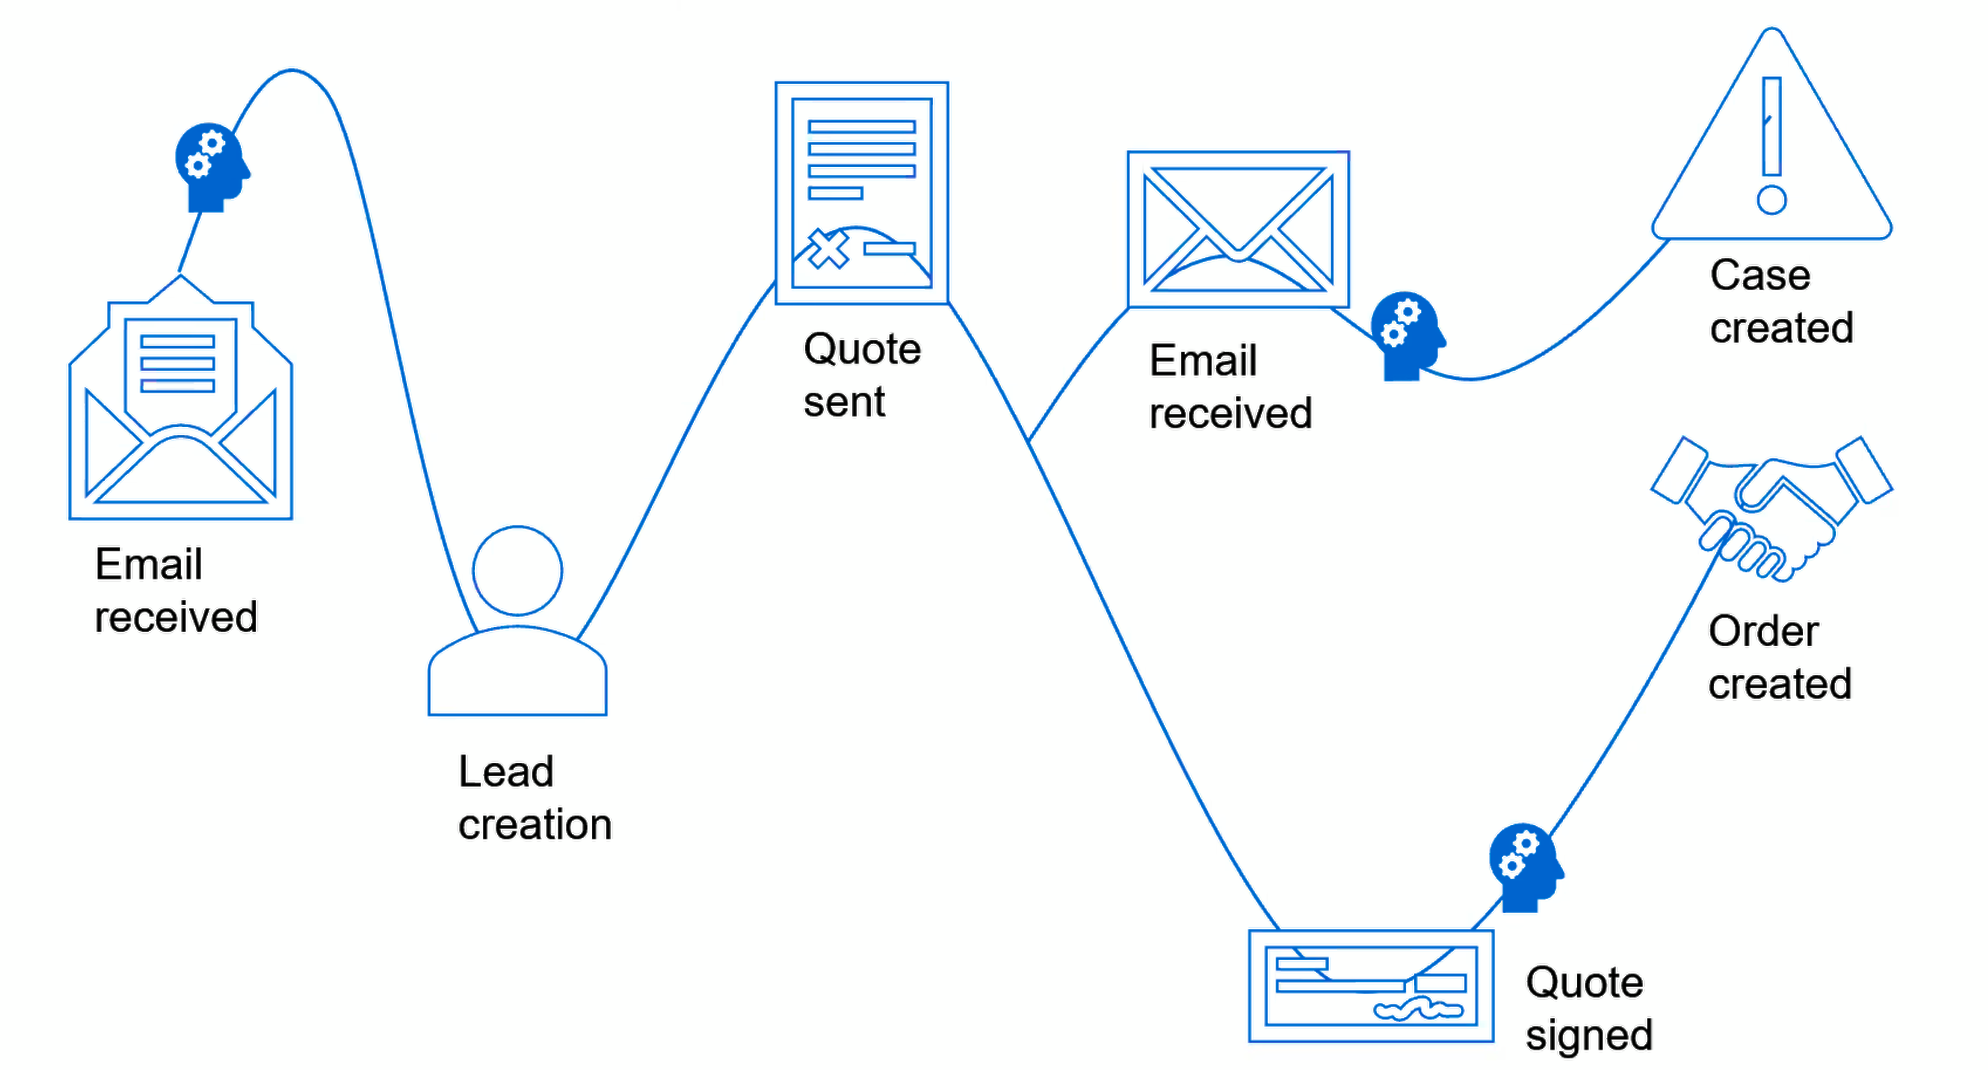
\includegraphics[width=0.8\textwidth]{processo-utilities.png}
  \caption{Processo di business modellato dal progetto.}
  \label{fig:processoUtilities}
\end{figure}

Nel dettaglio si compone dei seguenti passaggi:
\begin{enumerate}
  \item Arrivo di un email da parte di un potenziale cliente con in allegato un modulo compilato. Il modulo contiene informazioni riguardanti il cliente stesso (anagrafica) e le necessità di fornitura di energia per le quali ha effettuato la richiesta di preventivo.
  \item Il documento viene processato automaticamente mediante AI Builder e viene creato un nuovo record Lead nel CRM. Nel caso in cui il documento non venga processato correttamente o si verifichino errori viene inviata una email di cortesia al potenziale cliente che notifichi l'errore.
  \item In seguito alla creazione del Lead quest'ultimo viene automaticamente \textit{qualificato} in un record Opportunity mediante un Plugin.
  \item Un operatore compila manualmente il preventivo (Quote) di fornitura basandosi sui dati raccolti in precedenza. 
  \item  Quando il preventivo viene contrassegnato come ''attivo'', viene avviato un secondo plugin che invia automaticamente un'email al cliente contenente il preventivo come allegato.
  \item 
  \begin{itemize}
    \item Se il cliente risponde all'email con il preventivo firmato (con il controllo effettuato automaticamente grazie a un modello AI Builder), il Quote si considera vinto e viene convertito in Order per poi essere ultimato da un operatore. 
    \item Se il cliente risponde all'email in qualsiasi altro modo, un modello di classificazione di categoria di AI Builder analizza il testo dell'email. Sulla base dell'output di questo modello, viene creato un record Case e assegnato a un'apposita coda del modulo funzionale Service per essere processato da un operatore.
  \end{itemize}
\end{enumerate}

\section{Sviluppo del progetto}
In seguito alla definizione dettagliata dei requisiti ho proceduto con lo sviluppo del progetto che ha richiesto l'utilizzo di Power Automate, AI Builder, Plugin e customizzazioni di form e regole di \textit{routing} per l'instradamento dei Case nelle varie Queue.

\subsection{AI Builder}
Sono stati utilizzati due diversi tipi di modelli AI Builder:
\begin{itemize}
  \item Modello personalizzato per l'elaborazione di moduli - utilizzato per l'estrazione di dati dal modulo di richiesta preventivo e per verificare l'accettazione del preventivo.
  \item Modello predefinito di classificazione delle categorie per classificare il contenuto dell'email di risposta all'invio del preventivo.
\end{itemize}

\subsubsection{Modulo di richiesta preventivo}
Avendo praticamente carta bianca su come sviluppare il modulo ho potuto evitare le problematiche riscontrate durante il primo progetto. In Figura~\ref{fig:moduloRichiestaPreventivo} un esempio di modulo. Per questo progetto, come indicato dal mio supervisore, non mi sono soffermato in modo eccessivo sul training del modello e ho utilizzato semplicemente un campione di \num{5} documenti compilati. Per brevità, inoltre, non riporto l'elenco dei campi riconosciuti, in quanto corrispondono alle celle compilabili del documento in Figura~\vref{fig:moduloRichiestaPreventivo}.

\begin{figure}[ht!]
  \centering
    \subfloat[][\emph{Pagina 1.}]
       {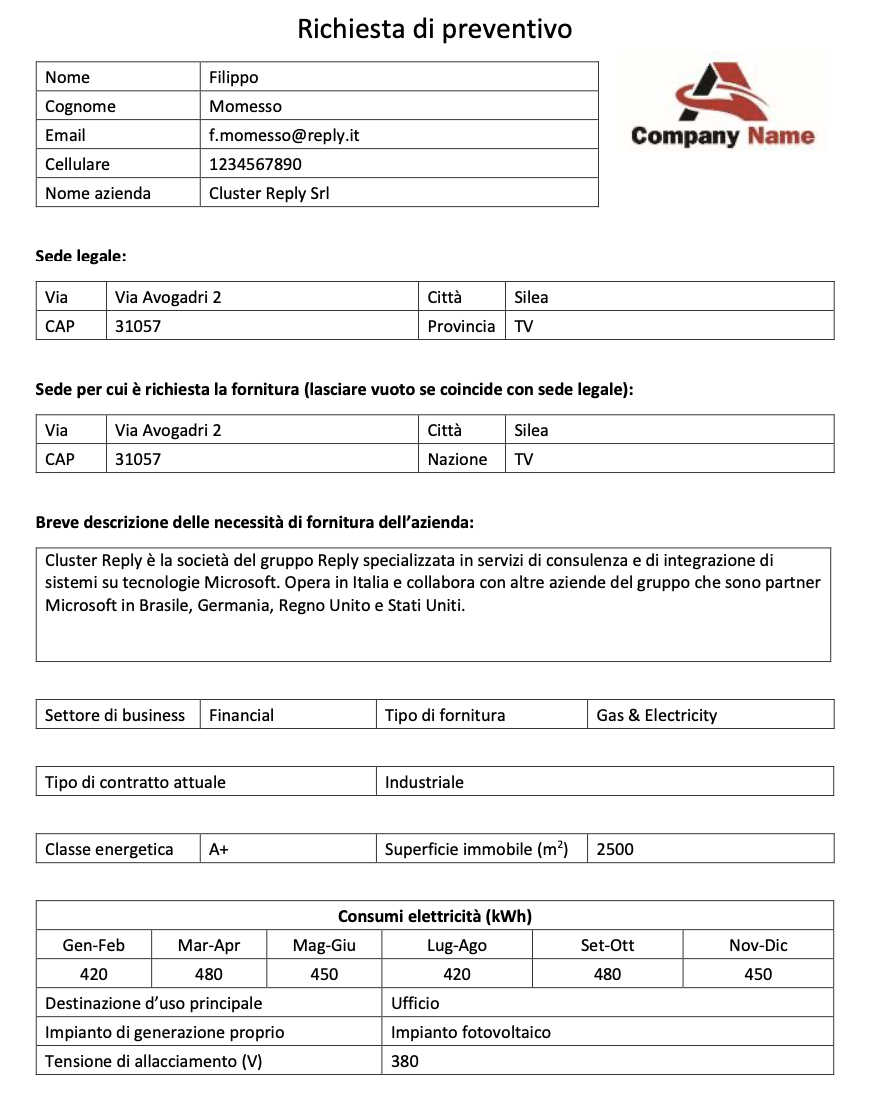
\includegraphics[width=.45\textwidth,valign=c]{modulo-richiesta-preventivo1.png}} \quad
    \subfloat[][\emph{Pagina 2.}]
       {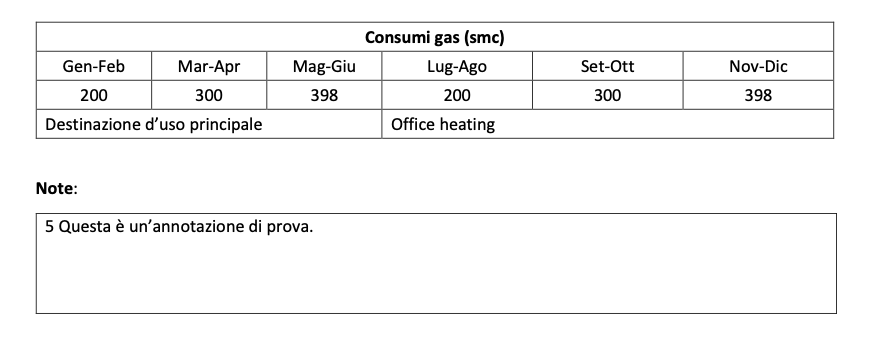
\includegraphics[width=.45\textwidth,valign=c]{modulo-richiesta-preventivo2.png}} \\
  \caption{Esempio di modulo utilizzato.}
  \label{fig:moduloRichiestaPreventivo}
\end{figure}

\subsubsection{Documento con preventivo accettato}
Per l'accettazione del preventivo si è optato per l'apposizione di data e firma. È stato dunque creato un modello di elaborazione di moduli che rilevasse nome del cliente, ID del Quote, data e firma. Tuttavia, come riportatato in Sezione~\ref{ssec:creazioneModello}, il rilevamento di firme non è ancora supportato da AI Builder ma stando a informazioni interne giunte a Cluster Reply, lo sarà in futuro. Pertanto, in fase di validazione del documento, la firma verrà semplicemente ignorata e i controlli verranno effettuati solamente sui restanti campi analizzati. In Figura~\ref{fig:documentoPreventivo} un esempio di documento utilizzato per questo modello. Anche in questo caso per il training è stato utilizzato un campione di \num{5} documenti compilati.

\begin{figure}[ht!]
  \centering
  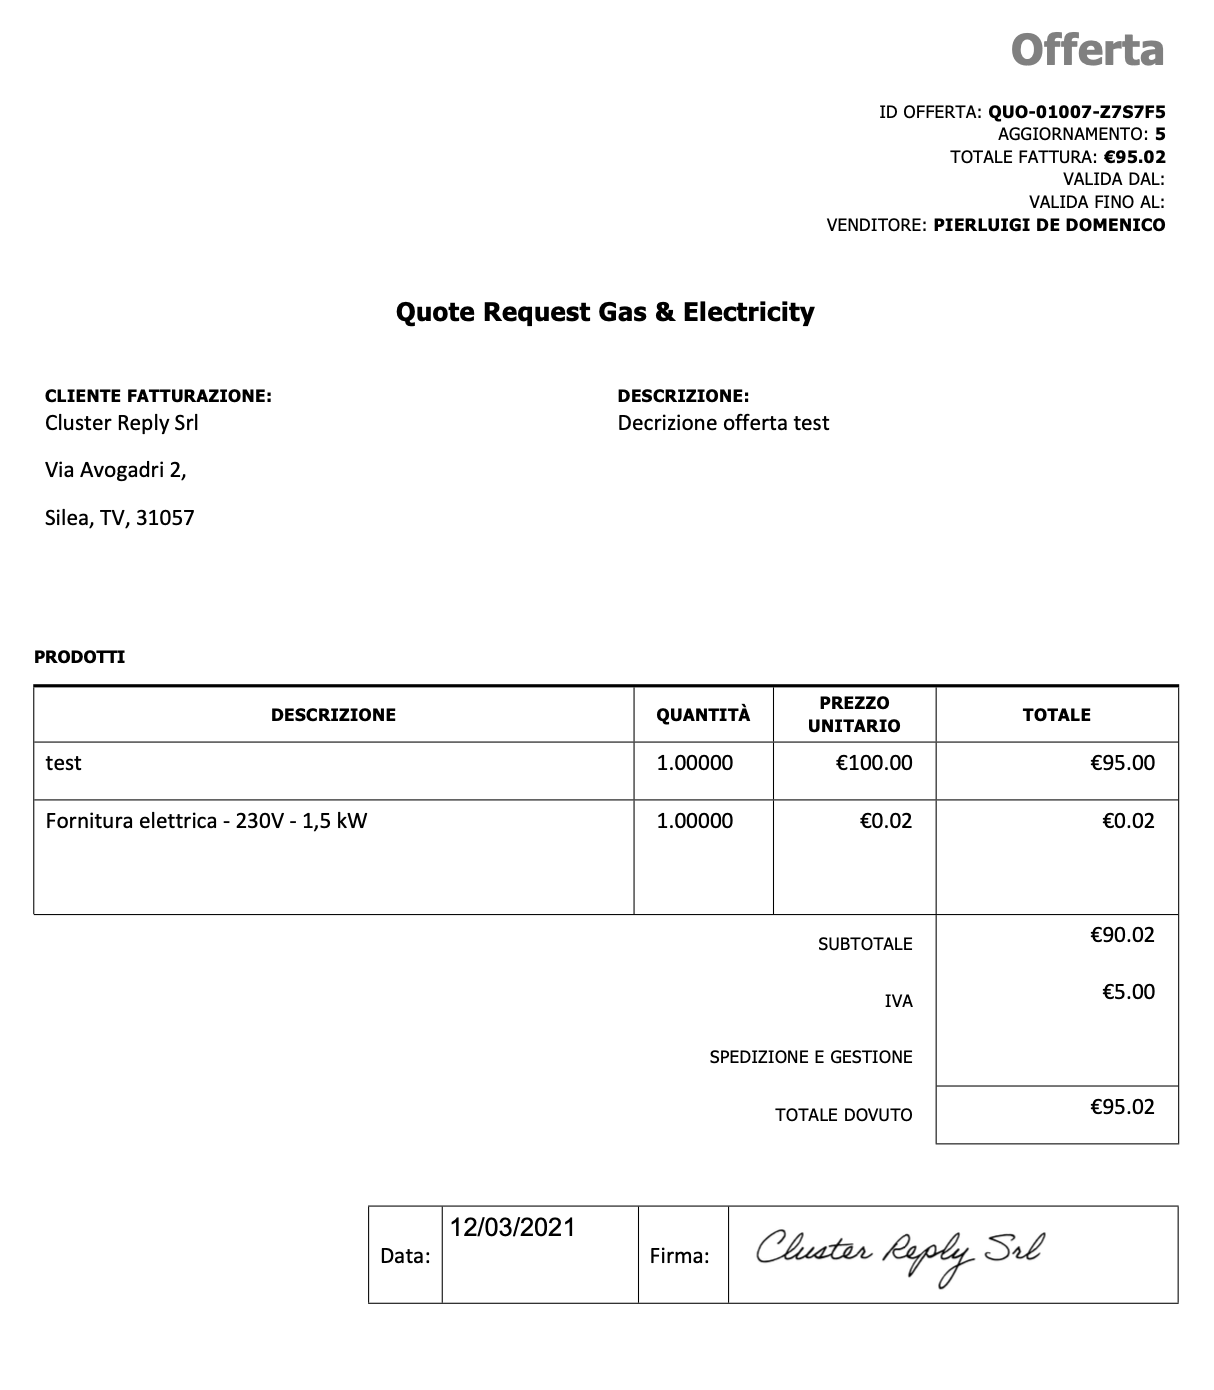
\includegraphics[width=0.5\textwidth]{documento-preventivo.png}
  \caption{Esempio di preventivo compilato e firmato per accettazione.}
  \label{fig:documentoPreventivo}
\end{figure}

\subsection{Flussi Power Automate}
Sono stati sviluppati due flussi cloud: il primo copre le fasi del processo che vanno dalla ricezione dell'email con allegato fino alla creazione del Lead; il secondo, invece, si occupa di gestire quanto avviene dopo l'invio del preventivo, ovvero la risposta positiva o negativa del cliente.

\subsubsection{Flusso di creazione del Lead}
In Figura~\ref{fig:flussoCreazioneLead} è riportato il primo flusso cloud sviluppato, il quale si occupa di creare il Lead a partire dai dati estratti dal documento ricevuto come allegato dell'email.

Si compone di diverse fasi:
\begin{enumerate}
  \item Trigger sulla creazione di un record Attachment.
  \item Controlli su destinatario dell'email e tipo di documento.
  \item Conversione del documento in PDF se l'allegato non è in formato PDF.
  \item Estrazione dei dati dal documento mediante modello AI Builder.
  \item Operazioni di validazione sui dati estratti
  \item Creazione del Lead e aggiornamento del campo Regarding dell'email in modo da associarla al Lead.
\end{enumerate}

\begin{figure}[ht!]
  \centering
  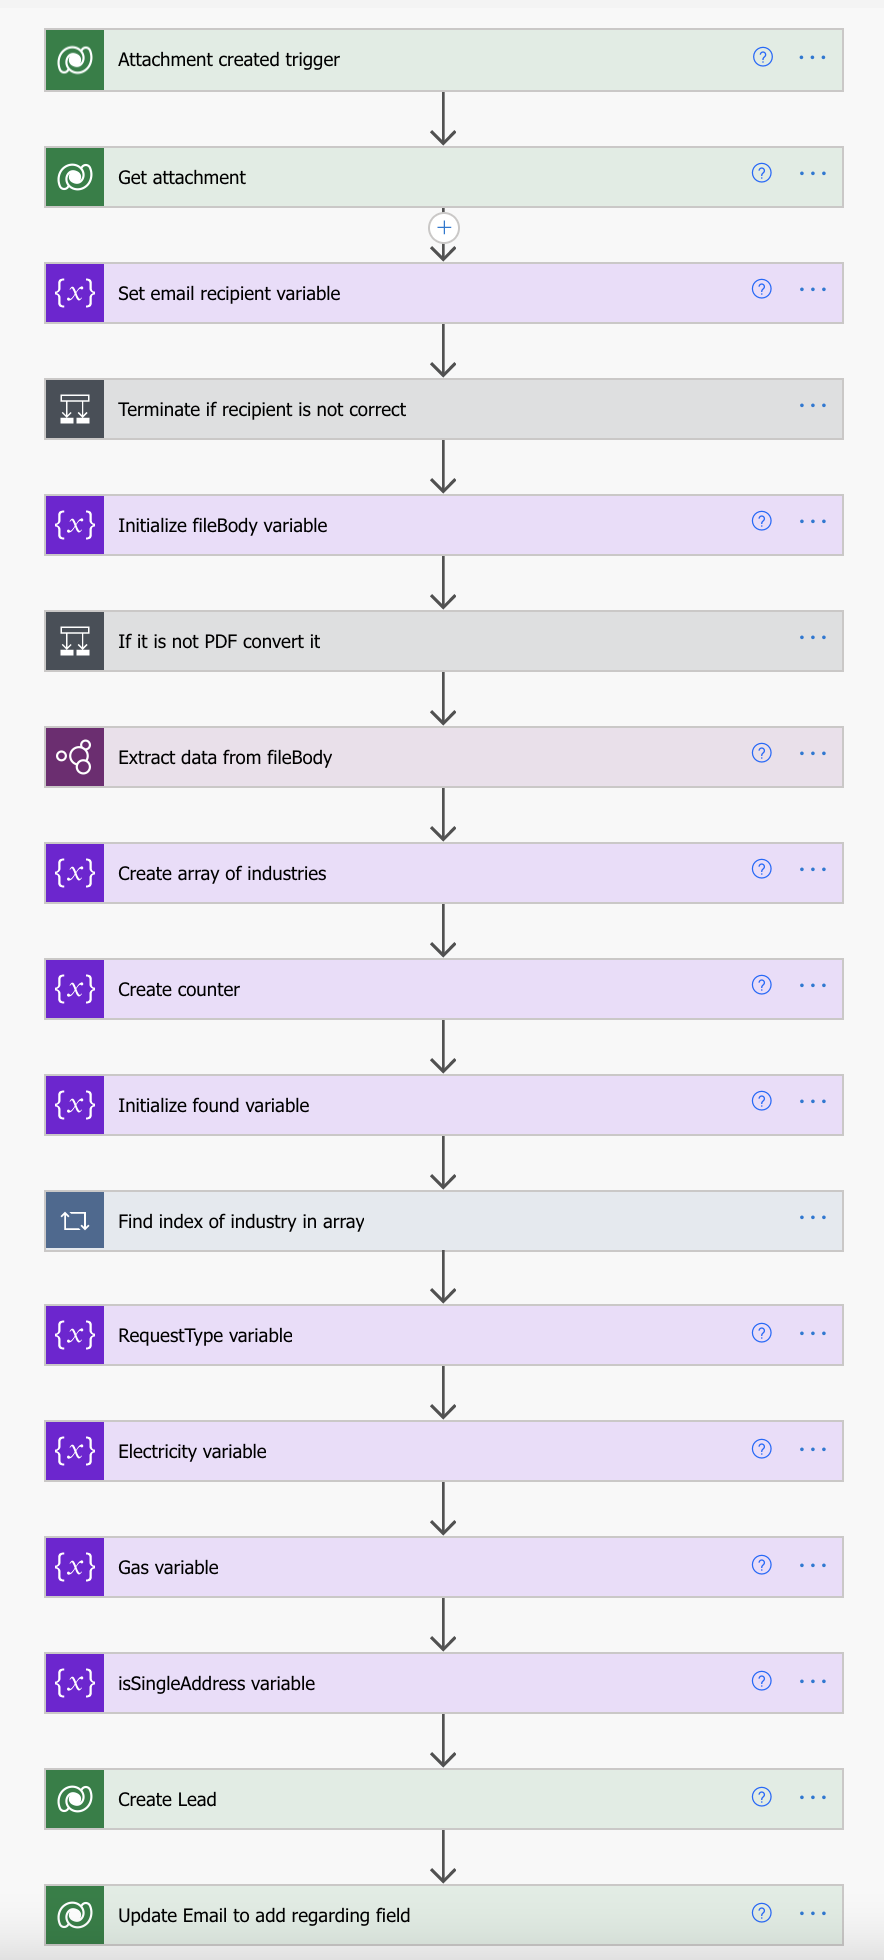
\includegraphics[width=0.45\textwidth]{flusso1.png}
  \caption{Flusso di creazione del Lead}
  \label{fig:flussoCreazioneLead}
\end{figure}

\subsubsection{Flusso di elaborazione della risposta del cliente}
Il flusso che viene eseguito in seguito alla ricezione di un email di risposta a un preventivo è più articolato in quanto necessita di gestire due possibilità: offerta accettata oppure offerta rifiutata.

Si compone delle seguenti fasi:
\begin{enumerate}
  \item Trigger sulla creazione di un record Email e controllo che l'email sia associata ad un record Quote. Il CRM si occupa in automatico di creare le relazioni se un'email viene ricevuta come risposta ad un'email associata ad un record mediante il campo Regarding.
  \item Recupero di un eventuale allegato. Se presente il processo procede con:
  \begin{enumerate}
    \item Conversione del documento in formato PDF se non è in formato PDF.
    \item Estrazione dei dati dal documento mediante modello AI Builder.
    \item Validazione sui dati estratti con controllo sulle confidence. Un valore medio di confidence sui valori riconosciuti inferiore a \num{0.7} rende non valido il documento.
    \item Se il documento è valido e firmato, il Quote è considerato vinto e pertanto convertito in Ordine.
  \end{enumerate}
  \item Se il documento non è presente o risulta non valido, segue l'analisi del testo dell'email mediante il modello di classificazione di categorie.
  \item Creazione del Case il cui campo Description contiene l'output del modello utilizzato nella fase precedente e aggiornamento del campo Regarding dell'email in maniera tale da associarla al Case appena creato.
\end{enumerate}

\subsection{Plugin}
Sono stati sviluppati due Plugin che svolgono le seguenti operazioni: 
\begin{itemize}
  \item Conversione del Lead in Opportunity.
  \item Invio automatico di email con preventivo in allegato.
\end{itemize}

Come strumenti di sviluppo ho utilizzato Microsoft Visual Studio unitamente a Microsoft XRM Toolbox, utile per il debugging e la registrazione dei plugin nella soluzione del CRM.

\subsubsection{Conversione del Lead in Opportunity}
\label{ssec:conversioneLead}
Per la conversione del Lead in Opportunity ho scelto di utilizzare un Plugin registrato sul Create Message in fase Post-operation dell'entità Lead. In questo modo la sua esecuzione viene avviata al termine della creazione del Lead.

Mediante un'istanza di \lstinline[language={[Sharp]C}]{IOrganizationService} si ottiene il contesto in cui il plugin viene eseguito, e in questo modo è possibile, ad esempio, avere informazioni sul record che ha avviato l'esecuzione. La classe \lstinline[language={[Sharp]C}]{ITracingService} permette di stampare dei log sul CRM. 

Per prima cosa il codice effettua dei controlli sull'esistenza di un Account o Contact a cui associare l'Opportunity una volta convertita in Lead. Con la classe \lstinline[language={[Sharp]C}]{QueryExpression} è possibile, infatti, interrogare il CRM per ottenere dei record, come fosse una SELECT su un database. Nel Listato~\ref{QueryExpressionListing} un esempio di utilizzo.

\begin{lstlisting}[language={[Sharp]C},breaklines=true,caption={Esempio di utilizzo di una QueryExpression.},label=QueryExpressionListing]
  // Check if the account already exist 
  QueryExpression accountQuery = new QueryExpression("account");
  accountQuery.NoLock = true;
  accountQuery.ColumnSet = new ColumnSet("accountid");
  accountQuery.Criteria.AddCondition(new ConditionExpression("name", ConditionOperator.Like, companyName));
  if (partitaIva != null) accountQuery.Criteria.AddCondition(new ConditionExpression("accountnumber", ConditionOperator.Like, partitaIva));
  accountQuery.PageInfo.ReturnTotalRecordCount = true;
  EntityCollection resultsAccount = service.RetrieveMultiple(accountQuery);
\end{lstlisting}

Successivamente viene utilizzato un Message \lstinline[language={[Sharp]C}]{QualifyLeadRequest}, che fornisce la funzionalità standard di conversione di un Lead in Opportunity. A quest'ultimo vengono passati come parametri il Lead da qualificare ed eventuali riferimenti a Contact o Account se già esistenti a sistema. \lstinline[language={[Sharp]C}]{QualifyLeadRequest}, infatti, si occupa di default di creare Contact e Account per il potenziale cliente a partire dal Lead e, per evitare problemi con possibili duplicati, ho deciso di disabilitare il controllo automatico e gestire i duplicati manualmente. Il Listato~\ref{QualifyLeadRequestListing} riporta quanto appena spiegato.

Altre operazioni svolte sono l'aggiornamento di alcuni campi dell'Opportunity creatasi dopo l'esecuzione del suddetto Message.

\begin{lstlisting}[language={[Sharp]C},breaklines=true,caption={Utilizzo del Message QualifyLeadRequest.},label=QualifyLeadRequestListing]
  QualifyLeadRequest qualify = new QualifyLeadRequest {
    CreateOpportunity = true,
    OpportunityCurrencyId = currencyId,
    LeadId = new EntityReference(entity.LogicalName, entity.Id),
    Status = new OptionSetValue(OptionSet.Lead.StatusCode.Qualified)
  };

  if (contactExists && !accountExists) {
    // Create account and use existing contact as OpportunityCustomerId
    qualify.CreateAccount = true;
    qualify.OpportunityCustomerId = new EntityReference("contact", contactId);
  } else if (!contactExists && accountExists) {
    // Create contact and use existing account as OpportunityCustomerId
    qualify.CreateContact = true;
    qualify.OpportunityCustomerId = new EntityReference("account", accountId);
  } else if (contactExists && accountExists) {
    // Use existing account as OpportunityCustomerId
    qualify.OpportunityCustomerId = new EntityReference("account", accountId);
    //if contact is not associated to account 
  } else {
    qualify.CreateAccount = true;
    qualify.CreateContact = true;
  }

  //Disable DuplicateDetection
  qualify.Parameters.Add("SuppressDuplicateDetection", true);

  QualifyLeadResponse qualifyRes = (QualifyLeadResponse)service.Execute(qualify);
\end{lstlisting}

\subsubsection{Invio di email con preventivo}
\label{ssec:invioEmail}
Per l'invio automatico dell'email con il preventivo, ho deciso di utilizzare un Plugin registrato sull'Update Message in fase Post-operation dell'entità Quote. 

Per prima cosa viene controllato che il campo \textit{statecode} sia stato aggiornato ad \textit{attivo}, altrimenti l'esecuzione viene interrotta.
Dopodiché viene generato il documento PDF con il preventivo, codificato in formato \textit{base64}, mediante una chiamata all'Organization Web Service, come visibile nel Listato~\ref{OrganizationRequestListing}.

\begin{lstlisting}[language={[Sharp]C},breaklines=true,label=OrganizationRequestListing,caption=Chiamata all'azione ExportPdfDocument per la creazione del documento PDF.]
  private String generateEncodedPdf(IOrganizationService service, Entity quote, Guid documentTemplateId) {
      // Request to create pdf
      OrganizationRequest createPdfRequest = new OrganizationRequest("ExportPdfDocument");
      createPdfRequest["EntityTypeCode"] = 1084; // Quote typecode
      createPdfRequest["SelectedTemplate"] = new EntityReference("documenttemplate", documentTemplateId);
      createPdfRequest["SelectedRecords"] = "[\"{" + quote.Id.ToString() + "}\"]";

      OrganizationResponse createPdfResponse = (OrganizationResponse)service.Execute(createPdfRequest);

      return Convert.ToBase64String((byte[])createPdfResponse["PdfFile"]);
    }
\end{lstlisting}

Viene quindi creata l'email a partire da un template presente sul CRM. Per fare ciò prima si recupera il template attraverso una \lstinline[language={[Sharp]C}]{QueryExpression} e, successivamente, il template viene istanziato in un'email grazie a una chiamata al Message \lstinline[language={[Sharp]C}]{IstantiateTemplateRequest}. Nel Listato~\ref{GenerateEmailFromTemplate} è consultabile il codice corrispondente.
L'email viene poi completata con i valori \textit{destinatario} e \textit{mittente} e vien quindi creato un record Attachment sul CRM utilizzando il documento in formato \textit{base64} generato in precedenza.
Infine, l'email viene inviata mediante un Message \lstinline[language={[Sharp]C}]{SendEmailRequest}.

\begin{lstlisting}[language={[Sharp]C},breaklines=true,label=GenerateEmailFromTemplate,caption={Metodo per la creazione di un'email a partire da un template.}]
    //Create a query expression to get necessary email quote template
    QueryExpression queryBuildInTemplates = new QueryExpression {
      EntityName = "template",
      ColumnSet = new ColumnSet("templateid", "title"),
      Criteria = new FilterExpression()
    };
    queryBuildInTemplates.Criteria.AddCondition("title", ConditionOperator.Equal, "Template Offerta Email");
    EntityCollection templateEntityCollection = service.RetrieveMultiple(queryBuildInTemplates);

    Guid emailTemplateId = new Guid();

    if (templateEntityCollection.Entities.Count > 0) {
      emailTemplateId = (Guid)templateEntityCollection.Entities[0].Attributes["templateid"];
    } else {
      throw new ArgumentException("Standard Email Templates are missing");
    }

    // Create the request
    InstantiateTemplateRequest emailUsingTemplateReq = new InstantiateTemplateRequest {
      // Use a built-in Email Template of type "quote".
      TemplateId = emailTemplateId,

      // The regarding Id is required, and must be of the same type as the Email Template.
      ObjectId = quote.Id,
      ObjectType = "quote"
    };

    InstantiateTemplateResponse emailUsingTemplateResp = (InstantiateTemplateResponse)service.Execute(emailUsingTemplateReq);
\end{lstlisting}

\subsection{Gestione del Case}
Nell'eventualità che il flusso di elaborazione della risposta del cliente rilevi un documento non valido oppure non presente, procede con la creazione di un record Case la cui descrizione contiene l'output del modello di classificazione di categorie.
Le categorie possibili sono le seguenti:
\begin{itemize}
  \item Issues
  \item Customer Service
  \item Documentation
  \item Price \& Billing
  \item Compliment
  \item Staff
\end{itemize}

Per facilitare la gestione dei Case da parte degli addetti del settore Service ho creato quattro Queue, in cui i Case vengono distribuiti grazie a delle \textit{routing rules} (in italiano \textit{regole di instradamento}), una funzionalità del CRM che permette di redistribuire automaticamente i record in Queue sulla base di regole appositamente definite. In Tabella~\ref{table:routingRules} è possibile osservare come ho scelto di distribuire le sei tipologie di Case nelle rispettive Queue.

\begin{table}[ht]
  \centering
  \begin{tabular}{ll}
    \toprule
      \textbf{Tipologia di Case} & \textbf{Queue} \\ 
    \midrule
    Issues & \multirow{2}*{Problemi} \\
    Customer Service &  \\
    \midrule
    Documentation & Documentazione \\
    \midrule
    Price \& Billing & Prezzo e Fatturazione \\
    \midrule
    Compliment & \multirow{2}*{Generale} \\
    Staff &  \\
    \bottomrule
  \end{tabular}
  \caption{Tipi di Web Resource supportati}
  \label{table:routingRules}
\end{table}

\section{Considerazioni sul progetto}
Diversamente dal precedente, mi ritengo soddisfatto dell'esito di questo progetto. Salvo qualche intoppo durante lo sviluppo, risolto grazie all'aiuto dei colleghi più esperti, sono riuscito a portare a termine quanto richiesto e ho ottenuto un feedback positivo da parte del mio supervisore aziendale sul lavoro svolto. Quest'ultimo, inoltre, mi ha fatto sapere che, vista la qualità del risultato, sarebbe stato realmente utilizzato come \textit{demo} da mostrare ai potenziali clienti di Cluster Reply.



      
      
    \endgroup


    % bibliografia in formato bibtex
    %
    % aggiunta del capitolo nell'indice
    \addcontentsline{toc}{chapter}{Bibliografia}
    % stile con ordinamento alfabetico in funzione degli autori
    \bibliographystyle{plain}
    \bibliography{chapters/biblio/biblio}
%%%%%%%%%%%%%%%%%%%%%%%%%%%%%%%%%%%%%%%%%%%%%%%%%%%%%%%%%%%%%%%%%%%%%%%%%%
%%%%%%%%%%%%%%%%%%%%%%%%%%%%%%%%%%%%%%%%%%%%%%%%%%%%%%%%%%%%%%%%%%%%%%%%%%
%% Nota
%%%%%%%%%%%%%%%%%%%%%%%%%%%%%%%%%%%%%%%%%%%%%%%%%%%%%%%%%%%%%%%%%%%%%%%%%%
%% Nella bibliografia devono essere riportati tutte le fonti consultate 
%% per lo svolgimento della tesi. La bibliografia deve essere redatta 
%% in ordine alfabetico sul cognome del primo autore. 
%% 
%% La forma della citazione bibliografica va inserita secondo la fonte utilizzata:
%% 
%% LIBRI
%% Cognome e iniziale del nome autore/autori, la data di edizione, titolo, casa editrice, eventuale numero dell’edizione. 
%% 
%% ARTICOLI DI RIVISTA
%% Cognome e iniziale del nome autore/autori, titolo articolo, titolo rivista, volume, numero, numero di pagine.
%% 
%% ARTICOLI DI CONFERENZA
%% Cognome e iniziale del nome autore/autori (anno), titolo articolo, titolo conferenza, luogo della conferenza (città e paese), date della conferenza, numero di pagine. 
%% 
%% SITOGRAFIA
%% La sitografia contiene un elenco di indirizzi Web consultati e disposti in ordine alfabetico. 
%% E’ necessario:
%%   Copiare la URL (l’indirizzo web) specifica della pagina consultata
%%   Se disponibile, indicare il cognome e nome dell’autore, il titolo ed eventuale sottotitolo del testo
%%   Se disponibile, inserire la data di ultima consultazione della risorsa (gg/mm/aaaa).    
%%%%%%%%%%%%%%%%%%%%%%%%%%%%%%%%%%%%%%%%%%%%%%%%%%%%%%%%%%%%%%%%%%%%%%%%%%
%%%%%%%%%%%%%%%%%%%%%%%%%%%%%%%%%%%%%%%%%%%%%%%%%%%%%%%%%%%%%%%%%%%%%%%%%%
    

    \titleformat{\chapter}
        {\normalfont\Huge\bfseries}{Allegato \thechapter}{1em}{}
    % sezione Allegati - opzionale
    \appendix
    %\chapter{Titolo primo allegato}

Lorem ipsum dolor sit amet, consectetur adipiscing elit. Donec sed nunc orci. Aliquam nec nisl vitae sapien pulvinar dictum quis non urna. Suspendisse at dui a erat aliquam vestibulum. Quisque ultrices pellentesque pellentesque. Pellentesque egestas quam sed blandit tempus. Sed congue nec risus posuere euismod. Maecenas ut lacus id mauris sagittis egestas a eu dui. Class aptent taciti sociosqu ad litora torquent per conubia nostra, per inceptos himenaeos. Pellentesque at ultrices tellus. Ut eu purus eget sem iaculis ultricies sed non lorem. Curabitur gravida dui eget ex vestibulum venenatis. Phasellus gravida tellus velit, non eleifend justo lobortis eget. 

\section{Titolo}
Lorem ipsum dolor sit amet, consectetur adipiscing elit. Donec sed nunc orci. Aliquam nec nisl vitae sapien pulvinar dictum quis non urna. Suspendisse at dui a erat aliquam vestibulum. Quisque ultrices pellentesque pellentesque. Pellentesque egestas quam sed blandit tempus. Sed congue nec risus posuere euismod. Maecenas ut lacus id mauris sagittis egestas a eu dui. Class aptent taciti sociosqu ad litora torquent per conubia nostra, per inceptos himenaeos. Pellentesque at ultrices tellus. Ut eu purus eget sem iaculis ultricies sed non lorem. Curabitur gravida dui eget ex vestibulum venenatis. Phasellus gravida tellus velit, non eleifend justo lobortis eget. 

\subsection{Sottotitolo}
Lorem ipsum dolor sit amet, consectetur adipiscing elit. Donec sed nunc orci. Aliquam nec nisl vitae sapien pulvinar dictum quis non urna. Suspendisse at dui a erat aliquam vestibulum. Quisque ultrices pellentesque pellentesque. Pellentesque egestas quam sed blandit tempus. Sed congue nec risus posuere euismod. Maecenas ut lacus id mauris sagittis egestas a eu dui. Class aptent taciti sociosqu ad litora torquent per conubia nostra, per inceptos himenaeos. Pellentesque at ultrices tellus. Ut eu purus eget sem iaculis ultricies sed non lorem. Curabitur gravida dui eget ex vestibulum venenatis. Phasellus gravida tellus velit, non eleifend justo lobortis eget. 


\chapter{Titolo secondo allegato}

Lorem ipsum dolor sit amet, consectetur adipiscing elit. Donec sed nunc orci. Aliquam nec nisl vitae sapien pulvinar dictum quis non urna. Suspendisse at dui a erat aliquam vestibulum. Quisque ultrices pellentesque pellentesque. Pellentesque egestas quam sed blandit tempus. Sed congue nec risus posuere euismod. Maecenas ut lacus id mauris sagittis egestas a eu dui. Class aptent taciti sociosqu ad litora torquent per conubia nostra, per inceptos himenaeos. Pellentesque at ultrices tellus. Ut eu purus eget sem iaculis ultricies sed non lorem. Curabitur gravida dui eget ex vestibulum venenatis. Phasellus gravida tellus velit, non eleifend justo lobortis eget. 

\section{Titolo}
Lorem ipsum dolor sit amet, consectetur adipiscing elit. Donec sed nunc orci. Aliquam nec nisl vitae sapien pulvinar dictum quis non urna. Suspendisse at dui a erat aliquam vestibulum. Quisque ultrices pellentesque pellentesque. Pellentesque egestas quam sed blandit tempus. Sed congue nec risus posuere euismod. Maecenas ut lacus id mauris sagittis egestas a eu dui. Class aptent taciti sociosqu ad litora torquent per conubia nostra, per inceptos himenaeos. Pellentesque at ultrices tellus. Ut eu purus eget sem iaculis ultricies sed non lorem. Curabitur gravida dui eget ex vestibulum venenatis. Phasellus gravida tellus velit, non eleifend justo lobortis eget. 

\subsection{Sottotitolo}
Lorem ipsum dolor sit amet, consectetur adipiscing elit. Donec sed nunc orci. Aliquam nec nisl vitae sapien pulvinar dictum quis non urna. Suspendisse at dui a erat aliquam vestibulum. Quisque ultrices pellentesque pellentesque. Pellentesque egestas quam sed blandit tempus. Sed congue nec risus posuere euismod. Maecenas ut lacus id mauris sagittis egestas a eu dui. Class aptent taciti sociosqu ad litora torquent per conubia nostra, per inceptos himenaeos. Pellentesque at ultrices tellus. Ut eu purus eget sem iaculis ultricies sed non lorem. Curabitur gravida dui eget ex vestibulum venenatis. Phasellus gravida tellus velit, non eleifend justo lobortis eget. 




\end{document}
